\documentclass[11pt,a4paper,spanish,openright,twoside]{report}
\usepackage[spanish,activeacute,es-noquoting]{babel}
\usepackage[utf8]{inputenc}
\usepackage[top=2.25cm, bottom=2.25cm, outer=2.5cm, inner=2.5cm, heightrounded, marginparwidth=2.5cm, marginparsep=0.3cm]{geometry}

%load images
\usepackage{graphicx}
\graphicspath{{Images/}}

%math
\usepackage{amssymb}
\usepackage{amsmath}

%code snippets
\usepackage{listings}

%tikz pictures
\usepackage{tikz}
\usetikzlibrary{babel, decorations.pathreplacing, shapes, arrows, chains, patterns, trees, matrix, calc, mindmap} 
\usepackage{subfig}

%make figure stay in the declared position with H option
\usepackage{float}

%pie-charts
\usepackage{pgf-pie}

%\usepackage{smartdiagram}
%\usesmartdiagramlibrary{additions}

%Links in the document
\usepackage{hyperref} 
%Avoid numbers on blank pages
\usepackage{emptypage}
%To create list without indentation \begin{itemize}[leftmargin=*]
\usepackage{enumitem}
%Glossary
%\usepackage[acronym,toc]{glossaries}
\usepackage[toc,acronym]{glossaries}

%set document parameters
\addto\captionsspanish{\renewcommand{\contentsname}{\'{I}ndice General}}
\addto\captionsspanish{\renewcommand{\listfigurename}{\'{I}ndice de figuras}}
\addto\captionsspanish{\renewcommand{\listtablename}{\'{I}ndice de tablas}}
\addto\captionsspanish{\renewcommand{\appendixname}{Ap\'{e}ndice}}
\addto\captionsspanish{\renewcommand{\chaptername}{Cap\'{i}tulo}}
\addto\captionsspanish{\renewcommand{\tablename}{Tabla}}
\addto\captionsspanish{\renewcommand{\bibname}{Bibliograf\'{i}a}}
\addto\captionsspanish{\renewcommand{\glossaryname}{Glosario}}
\addto\captionsspanish{\renewcommand{\acronymname}{Acronimos}}

\makeindex

\makeglossaries

\newglossaryentry{oauth2}
{
  name=OAuth 2.0,
  description={OAuth 2.0 es un protocolo estándar de la industria para la autorización.
  OAuth 2.0 proporciona un flujo de autorización específico para aplicaciones web, de escritorio, dispositivos móviles\ldots}
}

\newglossaryentry{on-premise}
{
  name=On-premise,
  description={Software On-premise es instalado y ejecutado en el edificio (\textit{on the premises}) de la persona u organización que hace uso del software.}
}



\newacronym{xslt}{XSLT}{\textit{Extensible Stylesheet Language Transformations}}
\newacronym{erp}{ERP}{\textit{Enterprise Resource Planning}}
\newacronym{hrms}{HRMS}{\textit{Human Resource Management System}}
\newacronym{fms}{FMS}{\textit{Financial Management Solutions}}
\newacronym{scm}{SCM}{\textit{Supply Chain Management}}
\newacronym{crm}{CRM}{\textit{Customer Relationship Management}}
\newacronym{epm}{EPM}{\textit{Enterprise Performance Management}}
\newacronym{ceo}{CEO}{\textit{Chief Executive Officer}}
\newacronym{xml}{XML}{\textit{Extensible Markup Language}}
\newacronym{soap}{SOAP}{\textit{Simple Object Access Protocol}}
\newacronym{http}{HTTP}{\textit{Hypertext Transfer Protocol}}
\newacronym{wsdl}{WSDL}{\textit{Web Services Description Language}}
\newacronym{bnb}{BNB}{\textit{Business Network Builders}}
\newacronym{csv}{CSV}{\textit{Comma-Separated Values}}
\newacronym{api}{API}{\textit{Application Programming Interface}}
\newacronym{rest}{REST}{\textit{Representational State Transfer}}
\newacronym{json}{JSON}{\textit{JavaScript Object Notation}}
\newacronym{eib}{EIB}{\textit{Enterprise Interface Builder}}
\newacronym{mrp}{MRP}{\textit{Materials Requirement Planning}}
\newacronym{mrp2}{MRP II}{\textit{Manufacturing Resources Planning}}








%%%%%%%%%%REFERENCIAS%%%%%%%%%
%https://en.wikipedia.org/wiki/PeopleSoft





\begin{document}
	
	%title
	\begin{titlepage}
	\begin{center}

		% Upper part of the page. The '~' is needed because \\
		% only works if a paragraph has started.
		~\\[1.5cm]
		\textsc{\Large Integración de ERPs para Finanzas y RRHH\\ en entornos cloud}\\[1.5cm]

		{\Large Asier Cardoso Sánchez}\\[1.5cm]
        
        \textsc{\normalsize Doble grado en Ingeniería Informática y Matemáticas \\ Facultad de Informática \\ Universidad Complutense de Madrid}\\[1.5cm]
		
		
		\includegraphics[width=0.4\textwidth]{escudoUCM_color}\\[1.5cm]
        
        {\normalsize Trabajo de Fin de Grado}
		
		\vfill
		{\large \today}\\[1cm]
	\end{center}
    
    \begin{flushright}
        Directores:

        \ 
        
        Gonzalo Méndez Pozo
        
		Javier Delgado Taretto
    \end{flushright}
\end{titlepage}

	\chapter*{}
	\begin{flushright}
	\textit{Dedicado a \\
	mi familia}
	\end{flushright}
	%\input{Others/declaration.tex}
	\chapter*{Agradecimientos}
	\addcontentsline{toc}{chapter}{Agradecimientos} %evitamos que se numere
	Me gustaría agradecer a las personas que han hecho posible este trabajo:\\
	
	En primer lugar a Javier Delgado por permitirme la posibilidad de realizar este trabajo con un proyecto de Business Network Builders.
	También a Gonzalo Méndez que cuando le propuse ser mi tutor en el trabajo, aceptó encantado.\\

	A Carmen Fernández que fue la primera profesora con la que contacté para intentar realizar el trabajo en empresa.
	Gracias por resolverme esas dudas iniciales.\\
	
	Cómo no, también quiero mostrar mi agradecimiento a mi familia y a mi novia, 
	que han sabido soportarme en estos años de carrera y siempre que lo he necesitado han estado ahí para ayudarme.\\
	
	También quiero agradecer a todos los profesores que durante la carrera se han esforzado en enseñarnos la belleza de las matemáticas y la informática.\\
	
	Por último pero no por ello menos importante, quiero hacer un agradecimiento especial a mis compañeros, o mejor dicho amigos, de carrera.
	Con los que he compartido memorables experiencias durante estos cinco años. Sin duda alguna es una de las cosas más valiosas que me ha brindado la Universidad.\\
	
	
	\begin{center}
		\textit{Gracias}
	\end{center}
	
	
	
	

		

	
	\chapter*{Resumen}
	\addcontentsline{toc}{chapter}{Resumen} %evitamos que se numere
	
	Muchos estareis de acuerdo en que poder tener unificado en una aplicación multiples funcionalidades puede resultar una ventaja.
	Sin embargo hay ocasiones en las que esto no es posible, o poco conveniente si se trata de funcionalidades muy distintas.
	En estos casos nos vemos obligados a usar más de una aplicación que necesitan comunicarse y relacionarse entre sí.\\
	
	En estas situaciones, a pesar de que las aplicaciones suelen proporcionar herramientas que facilitan este trabajo, todavía se necesita desarrollar esta
	caja negra que sirva de puente entre ambas aplicaciones.\\
	
	Este trabajo de fin de grado se ha realizado en colaboración con una empresa.
	En este trabajo de fin de grado, se ha integrado dos aplicaciones cloud. El ERP Workday, él cual la empresa pretende empezar a usar,
	con el \gls{crm} Hubspot que se quiere continuar usando, él cual permite llevar un seguimiento de las oportunidades de negocio de la empresa.
	El trabajo consiste en el desarrollo de una interfaz que haga de puente entre ambas aplicaciones, 
	y conseguir la integridad de los datos entre las dos aplicaciones. \\
	
	
	Nuestro servicio estara escuchando aquellos mensajes que le lleguen desde Hubspot, para posteriormente tratarlos y comunicarse con Workday.
	De esta forma, cuando un deal u oportunidad de negocio se cree en Hubspot un mensaje llegará al servicio que lo procesará y enviará el correspondiente
	mensaje a Workday que refleje la creación de esa nueva oportunidad.\\
	
	
	Adicionalmente en el trabajo se ha hecho un estudio de los datos, de las diferentes oportunidades. Algunas de ellas convertidas en proyectos y otras con
	menos suerte que finalmente fueron oportunidades perdidas. El estudio tiene como intención el análisis de los datos de estas oportunidades,
	para que a partir de ellos se pueda predecir el resultado que se puede obtener con las oportunidades que están pendientes. 

	\
	
	\textbf{Palabras clave}
    
    Workday, Hubspot, Integration, \acrshort{erp}, \acrshort{crm}, Cloud, Analisis de datos, Machine learning.


\chapter*{Abstract}
	\addcontentsline{toc}{chapter}{Abstract} %evitamos que se numere
	Most of you probably agree that is better to have together in one application several funcionalities, than having them all separated in multiple ones.
	But there are some cases in which is not possible to acomplish that, or maybe it's not recommended. 
	In these situations we are forced to use multiple applications that should communicate between them.
	Applications usually provide services to make easier these integrations. Even though it's still necessary a lot of work to be done, in order to build this black box that will serve as bridge between the applications.\\
	
	This project has been carried out in collaboration with a company.
	In this final degree project, I have integrated two cloud applications. One of them is Workday a relatively recent ERP cloud based. 
	And the other is Hubspot a cloud CRM application to manage marketing and sales. Hubspot allows to have tracking of the different opportunities.\\
	
	Our interface will be listening to those messages coming from Hubspot, it will proccess them and then communicating with Workday.
	When a deal or business opportunity is created or modified in Hubspot, then our interface will received a message, after proccessing it,
	the interface will send a message to Workday to execute the corresponding operations to the project related to the Hubspot deal.\\
	
	Besides in this project, I have studied the data of the different opportunities.
	Some of them has ended up with success, and they become a real project. And some others unluckily has ended up as lost opportunities. 
	The study has as aim to analyze the data of these opportunities, and be able to forecast the outcome of the pending opportunities.
	
	\
	
	\textbf{Keywords}
    
    Workday, Hubspot, Integration, \acrshort{erp}, \acrshort{crm}, Cloud, Data analysis, Machine learning.
	
	

	
	\tableofcontents 
	\listoffigures
	\listoftables
	
	\chapter{Introducción}


\section{Motivaciones}
Este trabajo de fin de grado se ha realizado en colaboración con la empresa \acrfull{bnb}.
\acrshort{bnb} es una empresa de consultoría que proporciona a los clientes soluciones para distintas aplicaciones de negocio: \textit{SAP}, \textit{Workday}, \textit{PeopleSoft}, \textit{JD Edwards}.\\

Este trabajo de fin de grado es parte de un proyecto, concretamente es una de las integraciones de el proyecto.
El proyecto parte de la idea de mejorar el \textit{software} que se usa internamente para la parte de recursos humanos y finanzas. Se requiere facilitar las labores internas.
Comenzar a usar un \acrshort{erp} es una forma de conseguir reunir las funcionalidades de recursos humanos y finanzas en una aplicación.
Dado que \wday{} es un \acrshort{erp} moderno y opera en la nube, se trata de la opción que más encaja para la empresa y la que se decidió.
\\

Una vez fijado el proyecto surgen infinidad de tareas. Configurar \wday{} con todas las opciones y funcionalidades que desea tener la empresa, migrar los datos de aplicaciones previas como \textit{QlikView}, \textit{CM Plan}, 
integrar \wday{} con otras aplicaciones con las que tiene que coexistir cuando se salga a producción \ldots\\

Las aplicaciones que se deben integrar con \wday{} son \textit{Mantis Bug Tracker} y \hs{}.

Este trabajo de fin de grado consiste en la integración de \wday{} con \hs{}.

\hs{} es el \acrshort{crm} que usa actualmente la empresa y quiere mantenerlo tras la salida a producción.\\


El proceso de salida a producción debe ser rápido, ya que la empresa debe continuar con sus actividades empresariales. 
Es decir los procesos de migración y puesta en marcha de las integraciones tienen que hacerse en los dias previos a la slaida a producción.
Por ello , uno de los grandes retos que supone el proyecto es la salida a producción con el menor impacto posible a las actividades de la empresa.\\



Adicionalmente, por parte de la empresa se me solicitó hacer un prototipo de aplicación capaz de predecir la rotación de plantilla de la empresa.
Y así ser capaz de preveer cuando un empleado va a abandonar la empresa. \\

Con el desarrollo de este prototipo se quiere tomar las acciones necesarias para realizar una mejor predicción.



\section{Objetivos}

En esta sección vamos a establecer los objetivos a cumplir.

\begin{itemize}
	\item Desarrollar un microservicio que realice la integración entre \hs{} y \wday{}.
	\item Conseguir que al introducir datos en \hs{}, automaticamente se sincronicen con \wday{}.
	\item Que al modificar datos en \hs{}, se modifiquen en \wday{} de forma automática.
	\item Que la integración sea rápida, y el tiempo transcurrido entre la introducción o cambio de datos en \hs{} y los cambios en \wday{} sea el mínimo posible.
	\item La integración ha de ser segura. Estar provista de mecanismos para evitar posible ataques de terceras personas.
	\item La integración debe ser totalmente transparente para el usuario. 
	\item El programa no debe abortar su ejecución de manera inexperada.
	\item En la medida de lo posible evitar errores en la introducción de datos. Evitar que se cree información duplicada.
	\item El servicio que realiza la integración tiene que estar en ejcución ininterrumpida.
	\item Evitar la perdida de datos.
	\item Localmente se debe llevar la cuenta de los datos que se encuentran integrados.
	\item El servicio debe soportar ser reiniciado.
	\item El prototipo predictor debe ser capaz de decidir si es muy probable que un empleado abandone la empresa.
	\item Concluir que datos son más importantes para predecir el abandono en el trabajo.
	\item Poder tomar mediadas de acuerdo a las conclusiones a las que se llegue par elaborar mejores predicciones.
\end{itemize}


\section{Plan de trabajo}

Para la realización del proyecto de transición a \wday{} se ha seguido un sistema de metodología ágil. 
Cinco personas formabamos parte del equipo de proyecto y nos reuniamos al menos una vez por semana.
El proceso a durado unos tres meses y todos los integrantes realizabamos paralelamente tareas en otros proyectos.\\

En estas reuniones, se informaba de donde nos encontrabamos y cuales eran los siguientes pasos.
Por turnos se intervenía para explicar los avances que habíamos hecho hasta el momento y los problemas a los que nos estabamos enfrentando.
Las reuniones también servían para tomar decisiones sobre el proyecto.\\

En cuanto al desarrollo de la Interfaz de integración entre \hs{} y \wday{} se fue realizando de forma iterativa e incremental. 
Además, al tratarse de un grupo reducido, cualquier consulta o duda sobre los requisitos de la Interfaz podía ser solventada rápidamente.

Durante las últimas semanas se planificó mucho más detalladamente las tareas de cada uno, así como el momento en el que estas tareas debían ejecutarse.
Fue en estas últimas semanas cuando se necesitó la colaboración de otros compañeros de trabajo en el proyecto.\\

El desarrollo de la Interfaz de integración entre \hs{} y \wday{} se ha realizado de forma incremental.\\

En cada reunión se comunicaban los avances realizados y se proponían los ojetivos a cumplir para la próximo encuentro. Tras la reunion se comprobaban las nuevas funcionalidades implementadas.\\

En las semanas posteriores a la salida a producción, gracias a las observaciones e incidencias anunciadas por los usuarios,
se ha continuado modificando la Interfaz. 

	
\chapter{Integración}

En este capítulo vamos a ver como funciona el sitema de integración. Para ello explicaremos en detalle cada uno de los componentes del sistema.\\

Si nos fijamos en la Figura \ref{fig:general_diagram} podemos ver como la \iface{} actúa como puente entre \hs{} y \wday{}. 

\begin{figure}[H]
\centering

    
\pagestyle{empty}
\begin{tikzpicture}
  \path[mindmap,concept color=black,text=white]
    node[concept] {\Large \textbf{Interfaz}}
    [clockwise from=120]
    child[concept color=orange, text=black] {
      node[concept] {App HubSpot}
      [clockwise from=90, inner sep=0.1cm]
      child { node[concept] {\textbf{HubSpot}} }
    }
	child[concept color=blue!35!cyan, text=black] {
      node[concept] {\textbf{Workday}}
    }
    ;
\end{tikzpicture}



\caption{Diagrama general del sistema \protect\footnotemark{}} 
\label{fig:general_diagram}
\end{figure}

\footnotetext{Modificación del ejemplo de \href{http://www.texample.net/tikz/examples/computer-science-mindmap/}{\textit{Till Tantau}}}	

Explicaremos como funcionan \hs{} y \wday{}. Como están organizados y cual es su estructura. También explicaremos los métodos de integración con los que cuenta cada una de las aplicaciones.
Por último, explicaremos en detalle el diseño de la \iface{} así como sus características.\\

La \iface{} esta conectada tanto a \hs{} como a \wday. 

A \hs{} se conecta a través de una aplicación que necesitamos crear en \hs{} y la comunicación  puede ser bidireccional. De la \iface{} hacia \hs{} se hace mediante peticiones \acrshort{http} a la \acrshort{api} de \hs{}. 
La comunicación en la otra dirección se realiza mediante los webhooks declarados en la aplicación de \hs{}\\

Por otro lado está \wday{} cuya comunicación es unidireccional. Únicamente existe comunicación propiamente dicha de la \iface{} hacia \wday. \wday{} sí que responde a algunas peticiones \acrshort{http} con información, pero nunca inicia un mensaje hacia la \iface.

\section{\hs{}}
En esta sección vamos a describir toda la información que necesitamos saber sobre \hs{} para entender la Integración.

%El \acrshort{crm} \hs{} permite realizar integraciones gracias a su \acrshort{api} \acrshort{rest}.
Primero debemos tener en cuenta que \hs{} se encuentra organizado en objetos. Y toda la información almacenada en \hs{} pertenece a uno de los siguientes tipos de objetos:

\begin{itemize}
	\item \textit{Contacts} o Contacto
	\item \textit{Companies} o Compañía
	\item \textit{Deals} u Oportunidad
\end{itemize}

Cada objeto tiene una serie de propiedades por defecto a las que se pueden añadir propiedades personalizadas.
Es importante tener en cuenta las relaciones posibles entre los distintos tipos de objetos.

\begin{itemize}
	\item \textit{Contacts}
	\begin{itemize}
		\item Un contacto puede ser asociado con un único objeto compañía.
		\item Un contacto puede ser asociado con múltiples objetos oportunidad.
	\end{itemize}
	\item \textit{Companies}
	\begin{itemize}
		\item Una compañía puede estar asociada a múltiples contactos.
		\item Una compañía puede estar asociada a múltiples oportunidades.
	\end{itemize}
	\item \textit{Deals}
	\begin{itemize}
		\item Un \textit{deal} puede estar asociado a múltiples objetos contacto y a múltiples objeto compañía.
	\end{itemize}
\end{itemize}

En \hs{} un \textit{deal} puede estar asociado a una o más \textit{companies}. Para el caso de nuestra integración a lo sumo habrá un \textit{company} asociado a cada \textit{deal}.

Los objetos que nos interesan para nuestra integración son \textit{deal} y su \textit{company} asociado. La creación o modificación de un \textit{deal} iniciaran procesos de integración.



\subsection{Descripción del objeto \textit{Deal}}
	Es un objeto de \hs{} que representa una oportunidad de negocio con cierto cliente. Por defecto en \hs{} tenemos las siguientes propiedades asociadas a un deal:			
		\textit{Deal Id}, \textit{Amount}, \textit{Close Date}, \textit{Closed Lost Reason}, \textit{Closed Won Reason}, \textit{Create Date}, \textit{Deal Description}, \textit{Deal Name}, \textit{Deal Stage}, \textit{Deal Type}, \textit{Hubspot Owner}, \textit{Last Activity Date}, \textit{Last Modified Date}, \textit{Number of Contacts},
		\textit{Opp number}, \textit{Owner Assigned Date}, \textit{Pipeline}.
		
		Adicionalmente en la empresa se han creado propiedades personalizadas: \textit{Practice}, \textit{Transaction Amount}, \textit{Transaction Currency}.\\
		
		Las propiedades más importantes a tener en cuenta en la integración son las siguientes:
		\begin{itemize}
			\item \textbf{Deal id}: Identificador unívoco del \textit{deal} de \hs.
			\item \textbf{Close date}: Se trata de la fecha en la que se ha cerrado el acuerdo.
			\item \textbf{Deal Description}: Información describiendo el \textit{deal}.
			\item \textbf{Deal name}: Nombre del \textit{deal}.
			\item \textbf{Deal Stage}: estado en el que se encuentra el \textit{deal}. Esta se trata de una de las propiedades más importantes. 
				Esta propiedad puede tomar los siguientes valores.
				\begin{itemize}
					\item[$\circ$] Appointment Scheduled: Cuando se ha fijado una cita con el cliente.
					\item[$\circ$] Initial Contact: Si ya se ha tenido un primer contacto con el cliente.
					\item[$\circ$] Opportunity Identfied: En caso de que se haya identificado una oportunidad de negocio con el cliente.
					\item[$\circ$] Preparing Proporsal: Si se está preparando una proposición de oferta al cliente.
					\item[$\circ$] Proporsal Sent: Una vez se haya enviado la proposición de oferta al cliente.
					\item[$\circ$] Decision Maker Bought In: Una vez la oferta ya esta hecha y el cliente tiene la posibilidad de decidir si la acepta o no.
					\item[$\circ$] Contract Sent: Cuando el contrato se ha enviado al cliente.
					\item[$\circ$] Closed Won: Si la oportunidad de negocio se ha cerrado favorablemente.
					\item[$\circ$] Closed Lost: En caso de que se haya perdido la oportunidad con el cliente.
				\end{itemize}
		\end{itemize}
		
		
		Es de especial importancia la propiedad \textit{Deal Stage}, ya que dependiendo de su valor se realizará o no la sincronización.
		La propiedad \textit{Deal Stage} representa el estado en el que se encuentra un \textit{deal}.
		
		
		\begin{figure}[H]
\centering
\begin{tikzpicture}[
	scale=0.75,
	start chain=1 going below, 
	node distance=1mm,
	stage/.style={
		scale=0.75,
		on chain=1,
		rectangle,
		rounded corners,
		draw=black, 
		very thick,
		text centered,
		text width=8cm,
		minimum height=12mm
		},
	discovery/.style={
		fill=cyan!30
	},
	progress/.style={
		fill=blue!30
	},
	closure/.style={
		fill=green!30
	},
	phase/.style={
		scale=0.75,
		on chain=1,
		minimum height=12mm,
		text width=2cm,
		text centered
	},
	every node/.style={font=\sffamily}
]



% Discovery phase
\node [stage, discovery] (AS) {Appointment Scheduled};
\node [stage, discovery, continue chain=going below] (IC) {Initial Contact};
% Progress phase
\node [stage, progress] (OI) {Opportunity Identfied};
\node [stage, progress] (PP) {Preparing Proporsal};
\node [stage, progress] (PS) {Proporsal Sent};
\node [stage, progress] (DM) {Decision Maker Bought In};
\node [stage, progress] (CS) {Contract Sent};
% Closure phase
\node [stage, closure] (CW) {Closed Won};
\node [stage, closure] (CL) {Closed Lost};

\draw [
    thick,
    decoration={
        brace,
        mirror,
        raise=0.5cm
    },
    decorate
](AS.west) -- (IC.west) node[midway,xshift=-2cm] {descubrimiento}; 

\draw [
    thick,
    decoration={
        brace,
        mirror,
        raise=0.5cm
    },
    decorate
](OI.west) -- (CS.west) node[midway,xshift=-2cm] {Progreso}; 


\draw [
    thick,
    decoration={
        brace,
        mirror,
        raise=0.5cm
    },
    decorate
](CW.west) -- (CL.west) node[midway,xshift=-2cm] {Cierre};

\end{tikzpicture}
\caption{Estados por los que pasa un deal \protect\footnotemark{}}
\label{fig:deal_phases}
\end{figure}



\footnotetext{Modificación del ejemplo de \href{http://www.texample.net/tikz/examples/pera-model/}{\textit{Erno Pentzin}}}	
		
		
		Un \textit{deal} pasa por tres fases.
		
		\begin{enumerate}
			\item \textbf{Fase de descubrimiento}: Fase inicial del \textit{deal}. Cuando un \textit{deal} se encuentra en esta fase, no se sincroniza con \wday. La información del \textit{deal} solo reside en \hs.
			\item \textbf{Fase de progreso}: fase intermedia del proceso en la que todavía esta por decidir si la oportunidad se va a ganar o no. Todos los \textit{deals} en esta fase se mantienen sincronizados con el correspondiente proyecto de \wday.
			\item \textbf{Fase de cierre}: Fase final del proyecto. Una vez un \textit{deal} ha alcanzado esta fase, se excluye la oportunidad y no se continua sincronizando. Desde este momento se trata de manera independiente el proyecto en \wday{}, y el \textit{deal} no se modifica más. 
		\end{enumerate}
	
		La fase a la que pertenece el \textit{deal} depende de su estado. En la Figura \ref{fig:deal_phases} se puede ver a que fase pertenece cada estado.
		
		
		Todo \textit{deal} empieza con un estado perteneciente a la fase de descubrimiento, con el paso del tiempo puede ir pasando a la fase de progreso y finalmente todo \textit{deal} termina en uno de los dos estados de la fase de cierre: \textit{Closed Won} y \textit{Closed Lost}.\\
			
			
		Además de propiedades, los objetos pueden tener asociaciones. En el caso del deal puede tener una o más \textit{companies} asociadas. La \iface{}, dará por hecho que cada \textit{deal} está asociado a lo sumo a una \textit{company}.
			
		Desde el portal de \hs{} es posible tanto crear nuevos \textit{deals} como modificar cualquier propiedad a excepción del \textit{Deal Id}.
		
		Cuando seleccionamos la opción de creación de un \textit{deal} nos aparece un formulario como el de la Figura \ref{fig:create_deal}.
		
		\begin{figure}
			\centering
			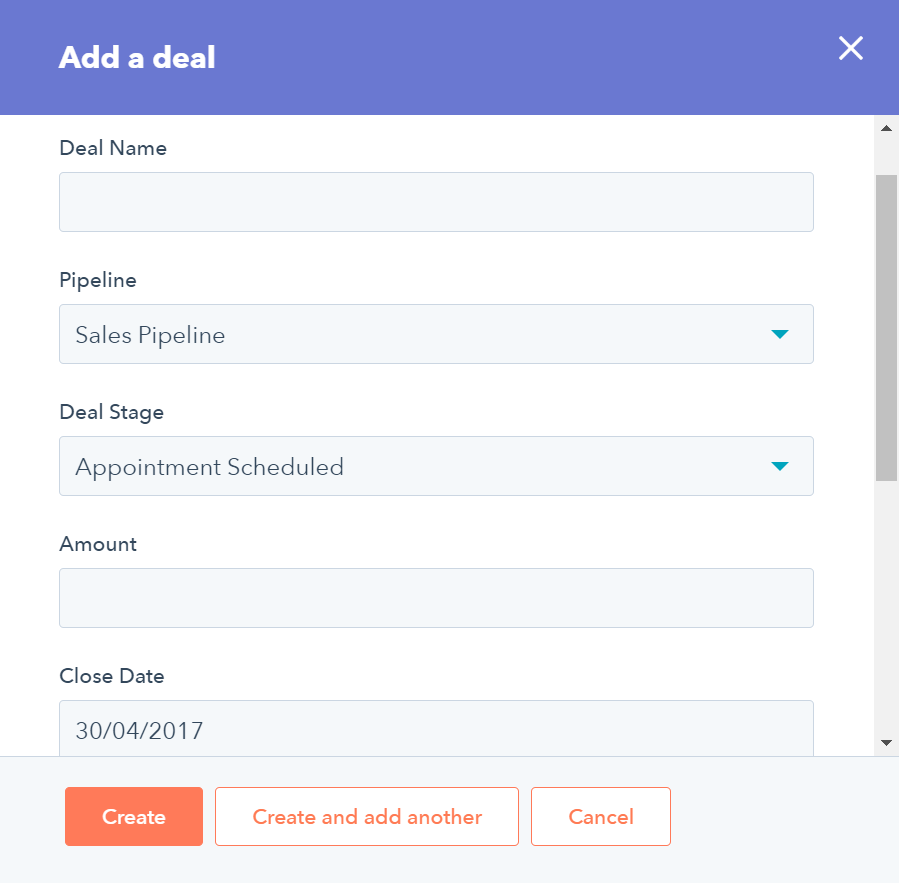
\includegraphics[width=0.5\textwidth]{deal_creation.png}
			\caption{Creando un \textit{deal} desde el portal de \hs{}}
			\label{fig:create_deal}
		\end{figure}

\subsection{Descripción del objeto \textit{Company}}
		
		Es un objeto de \hs{} que representa cualquier tipo de organización o empresa. 
		Este objeto cuenta con multitud de propiedades, que describen información de la empresa, como puede ser información de contacto, localización\ldots 
		
		Desde el portal de \hs{} es posible tanto crear nuevas \textit{companies} como modificar cualquiera de las ya existentes. Podemos ver el formulario de creación de una \textit{company} en la Figura \ref{fig:company_creation}.
		
		Sin embargo la creación o modificación de \textit{companies} no iniciarán procesos de sincronización. Solo se integrarán aquellas \textit{companies} que estén asociadas a un \textit{deal}.
		de esta forma evitamos que \textit{companies} con las que no existe un proyecto estén sincronizadas.
		
		\begin{figure}
			\centering
			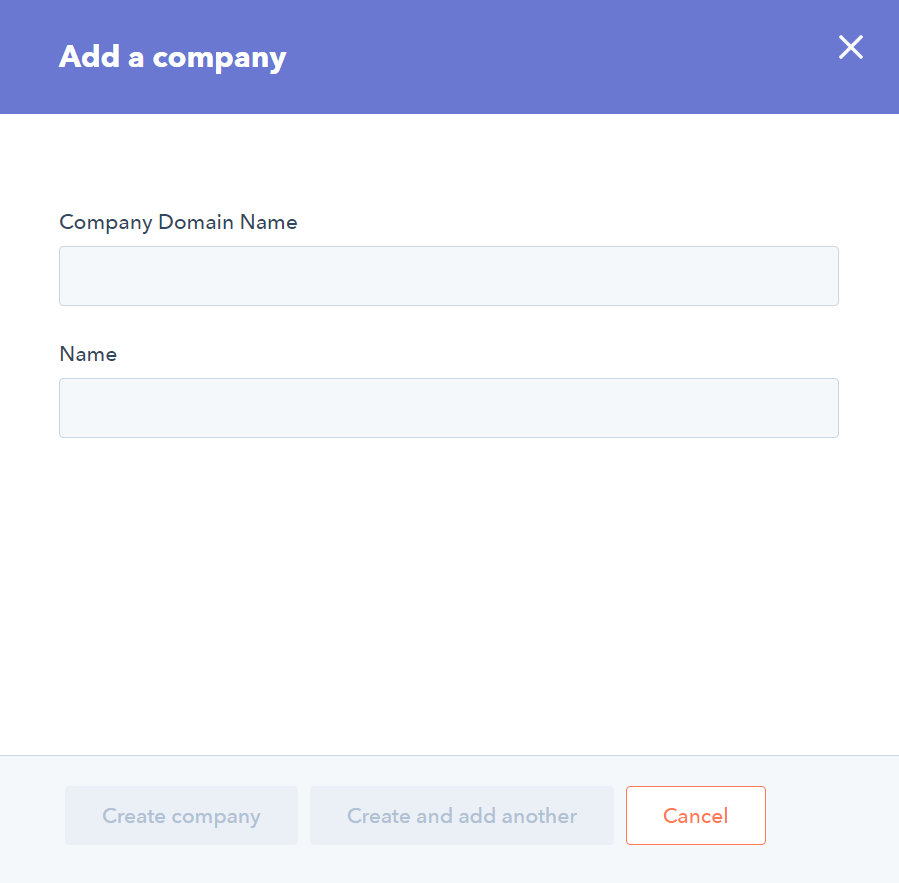
\includegraphics[width=0.5\textwidth]{company_creation.png}
			\caption{Creando una \textit{company} desde el portal de \hs{}}
			\label{fig:company_creation}
		\end{figure}


\subsection{Métodos de integración de \hs{}}
\hs{} cuenta con varios métodos para realizar las integraciones. Cada uno de ellos pensado para distintas situaciones.

\subsubsection{Integración con \textit{API keys}}

Para utilizar este método simplemente hay que consultar la clave de la \acrshort{api} de \hs{} (\textit{HAPIKey}), 
accesible desde el portal de \hs{} y añadirla como parámetro en las peticiones que enviemos al servicio \acrshort{rest} de \hs{}.\\

Este método es idóneo para realizar pruebas. Sin embargo su falta de seguridad impide su uso comercial. %Con este método no se puede garantizar la seguridad.

Además con este método solo es posible la comunicación en un sentido, desde la \iface{} hacia \hs{}.

\subsubsection{Integración con \textit{OAuth}}
\label{subsec:app_hs}

Para poder usar este método de integración es necesario crearse una cuenta de desarrollador. Con la cuenta de desarrollador podemos crear una \textbf{aplicación de \hs{}} y acceder a su panel de control. 

Desde el panel de control podemos ver toda la información de la aplicación. La información que necesitaremos es el identificador de la aplicación, la clave \texttt{Client Id} y la clave \texttt{Client Secret}.

Otra funcionalidad del panel de control es la posibilidad de configurar las suscripciones \textit{Webhook} de \hs{}, que permiten enviar de mensajes desde \hs{} a destinos externos cuando ciertos eventos ocurren.

También podemos hacer un seguimiento del funcionamiento de la aplicación desde el panel de control. \\

Lo primero que necesitamos es instalar la aplicación en el portal de \hs{}.

Para instalar la aplicación en el portal de \hs{} hay que seguir un proceso de autorización llamado \gls{oauth2}. Este proceso se ha automatizado e integrado en la \iface{} creada. 
Los pasos que hay que seguir son los siguientes \cite{hsapi}:
%JSON enviado por el webhook

\begin{enumerate}
	\item Dirigirse a la url de autorización \footnote{\url{https://app.hubspot.com/oauth/authorize?client_id=<client_id>&scope=contacts&redirect_uri=https://www.hubspot.com/} sustituyendo \texttt{<client\_id>} por el su valor}.
	Iniciar sesión en el portal de \hs{} y así autorizar la instalación de la aplicación. Cabe destacar que solo se puede acceder a dicha \textit{url} y por tanto instalar la aplicación si se cuenta con el \texttt{Client ID}. también se necesita un usuario del portal con permisos para poder instalar aplicaciones.
	Haciendo público el \texttt{Client ID} de la aplicación, esta puede ser instalada por cualquier persona en portales a los que tengan acceso. En nuestro caso este valor permanecerá en privado y solo nosotros haremos uso de la aplicación.
		
	\item Tras dar acceso al portal se te redirige a una página en la que aparece como parámetro de la \textit{url} un código.
	\item Mediante este código, el \texttt{Client ID} y el \texttt{Client secret} podemos obtener un token de sesión con una llamada a la \acrshort{api}.
	Tras hacer la petición a la \acrshort{api} de \hs{}, nos devolverá un mensaje \acrshort{json} con los siguientes valores.
		\begin{itemize}
			\item \texttt{access\_token} clave para realizar las peticiones a la \acrshort{api} de \hs{}.
			\item \texttt{refresh\_token} clave para conseguir nuevo par (\texttt{access\_token}, \texttt{refresh\_token}) cuando el \texttt{access\_token} ha expirado.
			\item \texttt{expires\_in} tiempo en milisegundos de validez del \texttt{access\_token}, por defecto son seis horas.
		\end{itemize}
	\item Cuando el \texttt{access\_token} haya expirado podremos llamar a otro \textit{end point} especificando el \texttt{refresh\_token} y recibiremos un mensaje de vuelta con otro nuevo \texttt{access\_token} y \texttt{refresh\_token}.
\end{enumerate}

Usando un \textit{token} válido podremos realizar peticiones a los distintos \textit{endpoint} \acrshort{rest} de \hs{}, es decir, la comunicación de la \iface{} a \hs{}.

Con este método se garantiza que los \textit{token} van variando como mínimo cada seis horas a diferencia del método de integración con \textit{API keys} en el que la  clave es fija y solo varía si lo hacemos manualmente. 

La aplicación instalada sirve como paso intermedio para las comunicaciones entre \hs{} y la \iface{}.

La comunicación en el otro sentido, de \hs{} hacia la \iface{} se hace gracias a la configuración de los \textit{webhook} de \hs{}.

Desde el portal podemos configurar las suscripciónes a los \textit{webhook}. Es necesario especificar la dirección (\textit{host} y puerto) donde deseamos que los mensajes sean enviados ante los diferentes eventos.\\

En el caso de nuestra aplicación está suscrita a los siguientes eventos:
\begin{itemize}
	\item \textbf{deal.creation}: Cuando un nuevo \textit{deal} es creado en \hs{} se envía un mensaje.
	\item \textbf{deal.propertyChanged} 
		\begin{itemize}
			\item \texttt{dealstage}: Cuando en un \textit{deal} de \hs{} se modifica el estado.
			\item \texttt{practice}: Cuando en un \textit{deal} de \hs{} se modifica la práctica.
			\item \texttt{hubspot\_owner\_id}: Cuando en un \textit{deal} de \hs{} se modifica su propietario.
			\item \texttt{closedate}: Cuando en un \textit{deal} de \hs{} se modifica la fecha de cierre.
			\item \texttt{description}: Cuando en un \textit{deal} de \hs{} se modifica la descripción.
			\item \texttt{dealname}: Cuando en un \textit{deal} de \hs{} se modifica el nombre.
			\item \texttt{transaction\_currency}: Cuando en un \textit{deal} de \hs{} se modifica la moneda.
			\item \texttt{legal\_entity}: Cuando en un \textit{deal} de \hs{} se modifica la entidad.
		\end{itemize}
\end{itemize}

La versión que se debe usar de \textit{OAuth} es \textit{OAuth2.0} ya que \hs{} en un futuro no dará soporte a las integraciones con \textit{OAuth1.0}.


\section{\wday{}}

En esta sección vamos a describir la información que necesitamos saber sobre \wday.

\wday{} es un \acrshort{erp} que internamente se encuentra organizado en objetos.
 
Los objetos que van a ser de interés para realizar la integración son:
\textit{Project}, \textit{Customer} y \textit{Hierarchy}.\\

Además cada uno de estos objetos cuenta con una serie de campos, que pueden incluso hacer referencia a otros objetos.
Un \textit{project} tiene un \textit{customer} puede tener asociado y también puede tener dos \textit{hierarchies} asociadas, una opcional y una principal.\\


Para realizar las integraciones, \wday{} proporciona un catálogo de servicios web basados en \acrshort{soap} (\textit{Workday Web Services} \cite{wws}). 
Mediante estos servicios podemos hacer que la \iface{} interactúe con \wday{}.

Cada servicio cuenta con un conjunto de operaciones que pueden ser llamadas mediante su \textit{end point}.


Lo siguiente que necesitamos saber es el formato de los mensajes que se deben enviar a estos \textit{end point}. Para ello contamos con el fichero \acrshort{wsdl} de cada servicio que especifica el formato de los mensajes \acrshort{soap} que se deben enviar para realizar cada operación.


El envío de los mensajes se realiza por \acrshort{http}.\\

Una herramienta que se ha utilizado para probar los servicio es \textit{SOAP UI}.

Además es necesario proporcionar credenciales en el mensaje para que \wday{} realice las operaciones deseadas.

Ante estas solicitudes \wday{} siempre responde indicando si la operación se ha realizado correctamente o el error que ha sucedido.



\subsection{Descripción del objeto \textit{Project} en \wday{}}
Es un objeto de \wday{} y existe una instancia por cada proyecto. Dentro de nuestra integración, 
el objeto \textit{Project} de \wday{} se corresponde con el objeto \textit{Deal} de \hs{}. 
De forma que por lo general las acciones sobre el objeto \textit{Deal} en \hs{} darán lugar a otros eventos
 sobre el objeto \textit{Project} de \wday{}.\\
 
Un objeto \textit{Project} puede ser creado de manera manual, pero en nuestra integración, esto se realizará mediante los servicios web.
Para crear o modificar un proyecto ya existente hay que enviar un mensaje \acrshort{soap} por \acrshort{http}. 
Para ello hay que usar la operación \texttt{Submit\_Project}  incluida en el servicio \texttt{Resource\_Management}.\\

El objeto \textit{Project} cuenta con multitud de campos, son de especial importancia los siguientes: 

\begin{itemize}
\item \textbf{\textit{Project name}}: Nombre del proyecto, está sincronizado con el nombre del \textit{deal} correspondiente.
\item \textbf{\textit{Start Date}}: Fecha de inicio, está sincronizado con con la propiedad \texttt{close\_date} del deal.
\item \textbf{\textit{Status}}: Estado del proyecto, existe una correspondencia con la propiedad \texttt{deal\_stage} del deal en \hs{}.
\item \textbf{\textit{Description}}: Descripción del proyecto. Este campo se encuentra sincronizado con la propiedad \texttt{description} del \textit{deal}.
\end{itemize}

Otros campos que hacen referencia a objetos son estos: 
\begin{itemize}
\item \textbf{\textit{Project Hierarchy}}: La Jerarquía principal del proyecto. Este campo está en directa relación con la propiedad personalizadas
\texttt{practice} de \hs.
\item \textbf{\textit{OptionalProject Hierarchy}}: La jerarquía opcional del proyecto. Este campo se encuentra directamente relacionado con la propiedad \texttt{hubspot\_owner\_id} del correspondiente \textit{deal}.
\item \textbf{\textit{Customer}}: El cliente del proyecto. Existe una correspondencia entre el cliente y la asociación \texttt{associated\_company} del \textit{deal} en \hs{}.

\end{itemize}



\subsection{Descripción del objeto \textit{Customer} en \wday{}}
Se trata de un objeto de \wday{} que representa a los clientes de la empresa. este objeto de \wday{} se encuentra relacionado con el objeto \textit{company} de \hs. 
Gracias a la \iface{}, cuando se realice la integración de un \textit{deal}, también se integrará la \textit{company} asociada.

Existen múltiples métodos para crear o modificar un \textit{Customer} en \wday{}, de forma manual, hojas de calculo para carga de datos \ldots

En nuestro caso la creación y modificación de un cliente se hace desde la \iface{}, 
mediante la operación \texttt{Put\_Customer} del servicio web \texttt{Revenue\_Management}.

\subsection{Descripción del objeto \textit{Hierarchy} en \wday{}}

El objeto \textit{Hierarchy} de \wday{} se encarga de representar jerarquías.
Es decir, representa información que se encuentra estructurada en forma de árbol.\\

En nuestro caso tenemos una jerarquía principal que organiza los proyectos según a que práctica pertenecen. 
(En el caso de nuestra empresa las distintas prácticas son: \textit{PeopleSoft}, \textit{SAP}, \textit{Cloud} \ldots).\\

También existen jerarquías opcionales para organizar los proyectos según su \textit{Customer Manager} y su \textit{Project Manager}.

\subsection{Servicios web de \wday{}}

Para hacer uso de los servicios web de \wday{}, primero debemos de contar con una cuenta del \textit{tenant} (o entorno) con permisos para el uso de los servicios web que se vayan a usar.

Una vez tengamos dicho usuario, podremos realizar las operaciones.\\

Los pasos para realizar una operación concreta son los siguientes:

\begin{enumerate}
	\item Determinar en que servicio se encuentra la operación deseada.
	\item Conseguir el archivo \acrshort{wsdl}. En este archivo podremos encontrar el formato de mensaje correcto para cada una de las operaciones disponibles en dicho servicio.
	\item Modificar la plantilla de mensaje con los parámetros deseados. 
	Para comprobar que el mensaje realiza la operación deseada correctamente podemos usar la aplicación \textit{SoapUI} \footnote{\url{https://www.soapui.org/}}. %\cite{soapui}.
	\textit{SoapUI} permite abrir esquemas \acrshort{wsdl}, modificar directamente la plantilla del mensaje para cualquier operación del servicio y enviar el mensaje.
	\item Enviar el mensaje \acrshort{soap} por \acrshort{http} con el método POST.
	\item comprobar que no ha habido errores con el mensaje de respuesta proporcionado por \wday.
\end{enumerate}

Para el tratamiento de los mensajes \acrshort{soap} se ha realizado del siguiente modo.
Se ha usado la libreria de \textit{python} \textit{lxml} \footnote{\url{http://lxml.de/}}. 
\begin{enumerate}
	\item Se genera el archivo \textit{xml} con ayuda de la librería \textit{lxml}. Este \textit{xml} cuanta con los parametros necesarios para la llamada al servicio web de \wday{}.
	
	\item Con el archivo \acrshort{xslt} correspondiente se transforma el \acrshort{xml} en el mensaje \acrshort{soap}.
\end{enumerate}

Cuando \wday{} responde con un mensaje \acrshort{soap}, la \iface{} recupera los valores del \acrshort{xml} con ayuda de la librería \textit{lxml}.

\section{\iface{}}


Para el desarrollo de la \iface{} he usado el lenguaje de programación \textbf{python}, con el \textit{IDE} \textbf{PyCharm}. La librería principal, bajo la que se sustenta el servidor es \textbf{\textit{web.py}}.
Alternativas a esta librería pueden ser los \textit{frameworks} \textit{Flask} o \textit{Django}.
\textit{Flask} es un \textit{microframework}, sería una buena alternativa si hubiese que elegir algo distinto a  \textbf{\textit{web.py}}.

\textit{Django} es idónea para proyectos mucho más grandes. Requiera de un proceso más avanzado antes de poder empezar a desarrollar la aplicación.

La ventaja de \textit{web.py} es lo ligera que es y la facilidad de ponerla en marcha.\\

La \iface{} se encuentra ejecutándose de manera continua en un servidor y está escuchando en un puerto los distintos mensajes que puedan llegar de \hs{}.
En el panel de control de la aplicación de \hs{}, explicado en la sección \ref{subsec:app_hs}, debemos especificar el \textit{host} y puerto del servidor que está ejecutando la \iface{}\\


En esta sección vamos a explicar detalladamente el funcionamiento de la \iface{}.

\subsection{Estructura de la \iface{}}
Vamos a describir como se encuentra estructurada nuestra \iface. Para ello podemos ver la Figura \ref{fig:project_structure}. 

El proyecto de \textit{python} se encuentra organizado en diferentes archivos subdirectorios.

\begin{itemize}

	\item [\textendash] \textbf{\textit{service.py}}: Se encuentra en el directorio raíz y se encarga de ejecutar la aplicación 
	y en este modulo está definida la función que se ejecuta al recibir un mensaje \textit{POST}. Desde este módulo se hacen llamadas a distintas funciones de \textit{handler.py}.
	\item [\textendash] \textbf{\textit{handler.py}}: También se encuentra en el directorio raíz y en este módulo se encuentra la lógica de programa para cada evento recibido.
	\item[\textendash] \textbf{\textit{hubspot}}: En este directorio se encuentran todos los módulos de \textit{python} que implementan funcionalidades para interactuar con \hs.
	
		\begin{itemize}
			\item [\textendash] \textbf{\textit{deal.py}}: En este módulo se encuentra la clase \textit{Deal}, encargada de representar en la \iface{} el objeto \textit{deal} de \hs.
			\item [\textendash] \textbf{\textit{company.py}}: En este módulo se encuentra la clase \textit{Company}, que se encarga de representar al objeto \textit{company} de \hs{}.
			\item [\textendash] \textbf{\textit{authorization.py}}: En este módulo se encuentra la clase Authorization encargada de facilitar el flujo de aprobación \gls{oauth2} de \hs{} y la renovación de los \textit{token} de sesión.
		\end{itemize}
		
	\item[\textendash] \textbf{workday}: En este directorio están los módulos encargados de la interacción con \wday.
	
		\begin{itemize}
			\item [\textendash] \textbf{\textit{project.py}}: En este módulo se encuentra la clase \textit{Project} que representa en la \iface{} el objeto \textit{Project} de \wday.
			\item [\textendash] \textbf{\textit{custommer.py}}: En este módulo se encuentra la clase \textit{Customer} que representa en la \iface{} el objeto \textit{Customer} de \wday.
			\item [\textendash] \textbf{\textit{hierarchy.py}}: En este módulo se encuentra la clase \textit{Hierarchy} que representa en la \iface{} el objeto \textit{Hierarchy} de \wday.
		\end{itemize}
	\item[\textendash] \textbf{modules}: En este directorio se encuentran agrupados módulos con funcionalidades diversas. 
	
			\begin{itemize}
				\item [\textendash] \textbf{\textit{configuration.py}}: En este módulo es donde inicializamos los \textit{Parser} de cada uno de los archivos de configuración.
				\item [\textendash] \textbf{\textit{database.py}}: Módulo para inicializar de las tablas de la base de datos y para la realización de operaciones en estas tablas.
				\item [\textendash] \textbf{\textit{log.py}}: Módulo encargado de implementar la salida a ficheros registro.
				\item [\textendash] \textbf{\textit{mail.py}}: Este módulo se encarga de la funcionalidad necesaria para enviar \textit{emails}.
			\end{itemize}
			
	\item[\textendash] \textbf{cfg}: En este directorio se encuentran todos los archivos de configuración. 
	Por lo general permanecen invariantes. A excepción de aquellos que almacenan \textit{tokens} de sesión que van cambiando.
	\item[\textendash] \textbf{xslt}: En este directorio se encuentran todas las plantillas de transformación necesarias para enviar los mensajes a \wday.
	Partiendo de un archivo \acrshort{xml}, podemos transformarlo con estas plantillas y generar un mensaje \acrshort{soap} para su posterior envío a \wday.
	

\end{itemize}

\begin{figure}
\centering
\tikzstyle{every node}=[draw=black,thick,anchor=west]
\tikzstyle{python}=[draw=blue,very thick, fill=blue!10, rounded corners]
\tikzstyle{folder}=[draw=orange,very thick,fill=orange!10]
%\tikzstyle{cfg}=[draw=red,fill=gray!50]
%\tikzstyle{xslt}=[draw=red,fill=gray!50]
\begin{tikzpicture}[
	scale=0.9,
  grow via three points={one child at (0.5,-1) and
  two children at (0.5,-1) and (0.5,-2)},
  edge from parent path={(\tikzparentnode.south) |- (\tikzchildnode.west)}]
	
	\node [folder]{ \Large Interfaz}
    child { node [python]{service.py}}		
    child { node [python]{handler.py}}
    child { node [folder] {hubspot}
      child { node [python]{deal.py}}
      child { node [python]{company.py}}
      child { node [python]{authorization.py}}
    }
	child [missing] {}				
    child [missing] {}				
    child [missing] {}
	child { node [folder] {workday}
      child { node [python]{project.py}}
      child { node [python]{customer.py}}
      child { node [python]{hierarchy.py}}
    }
	child [missing] {}				
    child [missing] {}				
    child [missing] {}
	child { node [folder] {modules}
      child { node [python]{configuration.py}}
      child { node [python]{database.py}}
      child { node [python]{log.py}}
	  child { node [python]{mail.py}}
    }
	child [missing] {}				
    child [missing] {}				
    child [missing] {}
	child [missing] {}				
	child { node [folder] {cfg}}
	child { node [folder] {xslt}};
	
	
	
\end{tikzpicture}
\caption{Estructura de la interfaz} \label{fig:project_structure}
\end{figure}


\subsection{Almacenamiento persistente}

En la \iface{} existen dos tipos de almacenamiento persistente: Estático y dinámico.

\begin{itemize}[leftmargin=*]
\item \textbf{Estático}: Se trata de los archivos de configuración ubicados en el directorio \textit{cfg} que se pueden ver en la Figura \ref{fig:project_structure}.
En estos archivos se guarda información como usuarios, contraseñas, \textit{token} de sesión, direcciones \textit{url}\ldots
De esta forma se evita que estos datos se encuentren \textit{Hardcodeados}. Nos facilita su modificación e
incluso la posibilidad de excluirlos fácilmente cuando se añada el proyecto a repositorios públicos.
Está información es fija (a excepción de los \textit{token} de sesión). Solo se cambiará cuando sea necesaria otra configuración.\\

Para su implementación he usado el módulo \textit{ConfigParser} \footnote{\url{https://docs.python.org/2/library/configparser.html}} parte de una librería estandar. \textit{ConfigParser} facilita la lectura de archivos de configuración. A estos archivos se les suele poner la extensión \textit{ini}. %TODO footnote cofigparser
Estos archivos de configuración se organizan en secciones formadas por listas de parejas clave-valor.
Una ventaja al usar \textit{ConfigParser} es que a la hora de definir una pareja clave-valor se puede referenciar un valor definido en la sección \textit{DEFAULT}. 


Otras alternativas para los archivos de configuración son \textit{yaml}, \textit{xml}, \textit{json}\ldots


\begin{itemize}
	\item [\textendash] \textbf{\textit{hubspot.ini}}: En este archivo se guarda la información referente a los \textit{tokens} de sesión, necesarios para comunicarse con el portal de \hs. 
	Este archivo cambia cada vez que se actualiza un \textit{token}.
	\item [\textendash] \textbf{\textit{workday.ini}}: En este archivo de configuración se 
	guardan las credenciales de acceso a \wday{}, así como distintas direcciones url para evitar su repetición en el código.
	\item [\textendash] \textbf{\textit{mapping.ini}}: En este archivo de configuración se encuentran todas las correspondencias entre \hs{} y \wday.
	\item [\textendash] \textbf{\textit{mail.ini}}: En este archivo de configuración se encuentran las credenciales necesarias para el acceso a la cuenta de correo.
\end{itemize}




\item \textbf{Dinámico}: Se trata de la base de datos local \textit{SQLite3} \footnote{\url{https://docs.python.org/2/library/sqlite3.html}} para \textit{python}. %TODO footnote sqlite3
 En esta base de datos se almacenan las distintas correspondencias entre \hs{} y \wday.
 
 Existen tres tablas en la base de datos: \texttt{deals\_excluded}, \texttt{deal\_project} y \texttt{company\_customer}.
 
 
 \begin{itemize}
	\item \texttt{deals\_excluded}: En esta tabla se almacena los identificadores de los \textit{deals} de \hs{} 
	que se encuentran excluidos para la integración. Todos los \textit{deals} que se encuentren en la fase de
	cierre estarán excluidos.
	\item \texttt{deal\_project}: En esta tabla se encuentra la correspondencias entre identificadores 
	de \textit{deals} de \hs{} y los identificadores de los \textit{projects} en \wday{}, para todos los \textit{deals} que han sido integrados.
	\item \texttt{company\_customer}: En esta tabla se encuentra la correspondencia entre las \textit{company} de \hs{} y los \textit{customers} de \wday{}
	para todos los \textit{companies} que hayan sido integrados.
 \end{itemize}
 

\begin{table}[H]
		\centering
		\begin{tabular}{
		|c|c@{\hskip 1cm} 
		|c|c|c@{\hskip 1cm} 
		|c|c|c@{\hskip 1cm}
		}
		\cline{1-1}\cline{3-4}\cline{6-7}
		deals\_excluded && \multicolumn{2}{c|}{deals\_excluded} && \multicolumn{2}{c|}{company\_customer} \\
	\cline{1-1}\cline{3-4}\cline{6-7}
	deal id && deal id & project id && company id & customer id \\
	\cline{1-1}\cline{3-4}\cline{6-7}
	\end{tabular}
	\caption{Tablas en la base de datos local}
	\label{tab:tables}
\end{table}

\end{itemize}




\subsection{Seguridad}
\label{subsec:security}

La \iface{} se encuentra escuchando los mensajes que le son enviados. Pero ¿Cómo podemos garantizar que el mensaje que recibimos proviene realmente de \hs{}?
Para ello existe un campo en la cabecera del mensaje recibido, que es \texttt{HUBSPOT\_SIGNATURE}. 
Este campo es el formado tras aplicar la función \textit{hash \textbf{sha256}} a la concatenación del \texttt{Client Secret} de nuestra aplicación de \hs{} con el cuerpo del mensaje \acrshort{http} recibido.\\

Basta hacer esta comprobación para garantizar la procedencia del mensaje, ya que el \texttt{Client Secret} solo es conocido por nosotros y por \hs{}. \\

Además cabe destacar que cualquier persona que interceptase el mensaje, no podría deducir el \texttt{Client Secret}, gracias a las propiedades de las funciones \textit{hash}. 

%TODO cite function hash


% A hash function is any function that can be used to map data of arbitrary size to data of fixed size. The values returned by a hash function are called hash values, hash codes, digests, or simply hashes. One use is a data structure called a hash table, widely used in computer software for rapid data lookup. Hash functions accelerate table or database lookup by detecting duplicated records in a large file. An example is finding similar stretches in DNA sequences. They are also useful in cryptography. A cryptographic hash function allows one to easily verify that some input data maps to a given hash value, but if the input data is unknown, it is deliberately difficult to reconstruct it (or equivalent alternatives) by knowing the stored hash value. This is used for assuring integrity of transmitted data, and is the building block for HMACs, which provide message authentication.

Como podemos comprobar en la Figura \ref{fig:validation_message}, aquellos mensajes que no cumplen los requisitos, se ignoran. Esto protege a nuestra \iface{} de aquellos mensajes no autorizados.

\begin{figure}
\centering

\shorthandoff{'}



\tikzstyle{line} = [draw, -latex']
\tikzstyle{startstop} = [rectangle, rounded corners, minimum width=3cm, minimum height=1cm,text centered, draw=black, fill=red!30]
\tikzstyle{io} = [trapezium, trapezium left angle=70, trapezium right angle=110, minimum width=3cm, minimum height=1cm, text centered, draw=black, fill=blue!30]
\tikzstyle{process} = [rectangle, minimum width=3cm, minimum height=1cm, text centered, draw=black, fill=orange!30]
\tikzstyle{decision} = [diamond, aspect=2,  minimum width=3cm, minimum height=1cm, text centered, draw=black, fill=green!30]
    
\begin{tikzpicture}[node distance = 3cm, auto]
	
	\node [io] (message) {Mensaje externo};
	\node [decision,below of =message] (valid) {¿Válido?};
	\node [startstop, below right of=valid, xshift=2cm, yshift=1cm] (no_valid) {Se ignora};
	\node [decision,below of =valid] (tipo) {¿Tipo?};
	
	\node [process, below left of=tipo, xshift=-2cm] (deal_creation) {Crear deal};
	\node [process, below right of=tipo, xshift=2cm] (deal_modification) {Modificar deal};
	
	\path [line] (message) -- (valid);
	\path [line] (valid.east) -| node {no}(no_valid);
	\path [line] (valid.south) -- node {sí}(tipo);
	
	\path [line] (tipo.west) -| node [left] {deal creation}(deal_creation);
	\path [line] (tipo.east) -| node {deal modfication}(deal_modification);
	
	
\end{tikzpicture}



\caption{Validación de los mensajes recibidos por la Interfaz} \label{fig:validation_message}
\end{figure}


\subsection{Flujo del programa}
%Dependiendo de de las acciones realizadas en \hs{}, se puede disparar un evento y que consiguientemente un mensaje se envíe a la \iface.

Como se ha mencionado anteriormente, nuestra aplicación de \hs{} está suscrita a diferentes eventos de los \textit{deals} de \hs{}.
Cuando uno de estos eventos se produce, la aplicación de \hs{} envía un mensaje \acrshort{http} (\textit{POST}) a la \iface{}. Este mensaje es un \acrshort{json} con información sobre el evento ocurrido. Podemos ver un mensaje de ejemplo en el Código \ref{lst:json_message}.\\

Para probar el correcto funcionamiento de la interfaz sin realizar cambio en \hs{}, se ha usado la herramienta \textit{cURL} \footnote{\url{https://curl.haxx.se/}}. 
Con \textit{cURL} podemos simular las peticiones \acrshort{http} enviadas desde \hs{}.

\begin{figure}
\begin{lstlisting}[caption={Ejemplo de mensaje recibido por la \iface{}},label={lst:json_message}, language=json]
	[{"objectId":92604011,
	  "changeFlag":"NEW",
	  "changeSource":"",
	  "eventId":2763628519,
	  "subscriptionId":1794,
	  "portalId":1234,
	  "appId":5678,
	  "occurredAt":1485865855549,
	  "subscriptionType":"deal.creation",
	  "attemptNumber":0}]
\end{lstlisting}
\end{figure}
 
Una vez recibido el mensaje se comprueba su validez verificando su procedencia como hemos visto en la Sección \ref{subsec:security}. Aquellos mensajes inválidos se ignoran como podemos ver en el diagrama de la \ref{fig:validation_message}.\\

Tras verificar que un mensaje es válido, se comprueba si dicho \textit{deal} se encuentra en la tabla de excluidos de base de datos local (\texttt{deals\_excluded}). 
Esta comprobación sirve como precaución para evitar la sincronización de proyectos no deseados en \wday{}.

Después dependiendo del valor del campo \textit{subscriptionType} comienza la ejecución de un proceso de creación de un deal o de modificación.

\begin{itemize}
	\item \textbf{Creación de un \textit{deal}}: Si el valor del atributo \textit{subscriptionType} es \textit{deal.creation}, éste nos indica que un \textit{deal} ha sido creado.
		En el mensaje \acrshort{json} también se especifica el id del \textit{deal} creado (\textit{objectId}) y otros datos de relevancia como el id del portal, id de la aplicación, momento en el que ocurrió el evento\ldots \\
	
		
		Los pasos que se siguen para el procesamiento del mensaje son los siguientes:
		
		\begin{enumerate}
			\item Se comprueba si el \textit{deal} está excluido, si es así entonces la petición no se procesa.
		
			\item Se comprueba si el \textit{deal} tiene una entrada en la tabla de correspondencias entre los \textit{deals} y \textit{projects} (\texttt{deals\_project}).
		En la tabla \texttt{deals\_project} se guarda la correspondencia entre los identificadores de los \textit{deals} de \hs{} y los identificadores de los \textit{projects} de \wday{} que están integrados.
		En caso de que el \textit{deal} esté en la tabla de correspondencias, quiere decir que el \textit{deal} se ha creado previamente y por tanto la petición se ignora y para el proceso.\\
		
		Si por el contrario no se encuentra en la tabla de correspondencias entonces se continua con el siguiente paso.
		
			\item Se realiza una petición a la \acrshort{api} de \hs{} para obtener el resto de información del \textit{deal} creado.
			\item Con todos los datos del \textit{deal} que se ha creado se comprueba si este se encuentra en la fase de progreso, en caso contrario dicho \textit{deal} no se integra y se para el proceso.
			\item Si el \textit{deal} se encuentra en la fase de progreso, entonces se comprueba si el \textit{company} asociado al \textit{deal} existe en la tabla de correspondencias entre los \textit{companies} y los \textit{customers} (\texttt{company\_customer}).
			En caso de que no exista se crea el correspondiente \textit{customer} en \wday{}, y se actualiza la tabla \texttt{company\_customer} con la nueva entrada .
			
			\item Se crea el \textit{project} asociándolo con el \textit{customer} previamente creado o existente y se actualiza la tabla \texttt{deals\_project} con la nueva correspondencia.
		\end{enumerate}
		
		
		
		\begin{figure}
\centering

\shorthandoff{'}



\tikzstyle{line} = [draw, -latex']
\tikzstyle{startstop} = [rectangle, rounded corners, minimum width=3cm, minimum height=1cm,text centered, draw=black, fill=red!30]
\tikzstyle{io} = [trapezium, trapezium left angle=70, trapezium right angle=110, minimum width=3cm, minimum height=1cm, text centered, draw=black, fill=blue!30]
\tikzstyle{process} = [rectangle, minimum width=3cm, minimum height=1cm, text centered, draw=black, fill=orange!30]
\tikzstyle{decision} = [diamond, aspect=2, minimum width=3cm, minimum height=1cm, text centered, draw=black, fill=green!30]
    
\begin{tikzpicture}[node distance = 3cm, auto]
	
	\node [startstop] (deal_creation) {Crear \textit{Deal}};
	\node [decision,below of =deal_creation] (db) {¿Está en BD?};
	\node [startstop, below right of=db, xshift=2cm, yshift=1cm] (in_db) {Se ignora el mensaje};
	\node [process,below of =db] (get_deal) {Obtener \textit{deal} de HubSpot};
	\node [decision,below of =get_deal] (valid) {\begin{tabular}{c}¿\textit{Dealstage} \\ válido? \end{tabular}};
	\node [process, below of=valid] (submit_customer) {Subir \textit{customer} a Workday};
	\node [process, below of=submit_customer] (submit_project) {Subir \textit{project} a Workday};
	
	
	\path [line] (deal_creation) -- (db);
	\path [line] (db.east) -| node {si}(in_db);
	\path [line] (db.south) -- node {no}(get_deal);
	\path [line] (get_deal.south) -- (valid);
	\path [line] (valid.south) -- node [left] {si} (submit_customer);
	\path [line] (valid.east) -| node [right] {no} (in_db);
	\path [line] (submit_customer.south) -- (submit_project);
	
	
\end{tikzpicture}



\caption{Proceso Crear Deal} \label{fig:deal_creation}
\end{figure}
		
		
	\item \textbf{Modificación de un \textit{deal}}:
	
		Si atributo \textit{subscriptionType} en el mensaje \acrshort{json} recibido tiene el valor \textit{deal.propertyChange}, quiere decir que se ha producido el cambio de alguna propiedad en un \textit{deal} de \hs{}.
		
		Los pasos que se siguen ante este tipo de mensajes son los siguientes:
		
		\begin{enumerate}
			\item Se comprueba si dicho \textit{deal} se encuentra en la tabla \texttt{deals\_excluded} de base de datos local. En tal caso, se para el proceso y no se sincronizan las modificaciones en \wday{}.
			\item Se comprueba si el \textit{deal} existe en la tabla de correspondencias \texttt{deal\_project}. De no ser así se procede a la creación del \textit{deal} con el proceso detallado anteriormente.
			\item Se obtiene el objeto \textit{project} de \wday{}. Se actualizan los correspondientes campos localmente, dependiendo de la propiedad del \textit{deal} que haya cambiado. Por último se actualiza el objeto \textit{project} correspondiente de \wday{} con los cambios realizados.
		\end{enumerate}
		
		
		
		Cuando un \textit{deal} pasa a un estado perteneciente a la fase de cierre, el \textit{deal} se añade a la tabla de excluidos \texttt{deals\_excluded}.
		
		
		\begin{figure}[H]
\centering

\shorthandoff{'}



\tikzstyle{line} = [draw, -latex']
\tikzstyle{startstop} = [rectangle, rounded corners, minimum width=3cm, minimum height=1cm,text centered, draw=black, fill=red!30]
\tikzstyle{io} = [trapezium, trapezium left angle=70, trapezium right angle=110, minimum width=3cm, minimum height=1cm, text centered, draw=black, fill=blue!30]
\tikzstyle{process} = [rectangle, minimum width=3cm, minimum height=1cm, text centered, draw=black, fill=orange!30]
\tikzstyle{decision} = [diamond, aspect=2, minimum width=3cm, minimum height=1cm, text centered, draw=black, fill=green!30]
    
\begin{tikzpicture}[node distance = 3cm, auto]
	
	\node [startstop] (deal_modification) {Modificar Deal};
	\node [decision,below of =deal_modification] (db) {¿Está en BD?};
	\node [process, below right of=db, xshift=2cm, yshift=1cm] (not_in_db) {Crear Deal};
	\node [process,below of =db] (get_deal) {Obtener deal de HubSpot};
	\node [process, below of=get_deal] (update_project) {Subir project en Workday};
	
	
	\path [line] (deal_modification) -- (db);
	\path [line] (db.east) -| node {no}(not_in_db);
	\path [line] (db.south) -- node {si}(get_deal);
	\path [line] (get_deal.south) -- (update_project);
	
	
\end{tikzpicture}



\caption{Proceso Modificar Deal} \label{fig:deal_modification}
\end{figure}

\end{itemize}




	\chapter{Predicción de abandono en el trabajo}

La empresa me solicitó realizar un prototipo que, partiendo de los datos de una plantilla de trabajadores, fuese capaz de predecir futuros casos de abandono en el trabajo.
Tras su dessarrollo se verían las posibilidades de integrarlo con \wday{}.\\

En este capítulo explicaremos en detalle los datos que vamos a utilizar. Estudiaremos estos datos y construiremos un modelo capaz de predecir cuando un trabajador va a abandonar el trabajo.\\




También se ha usado las librerías \textit{pandas}\footnote{\url{http://pandas.pydata.org/}} para la transformación y análisis de datos y la librería \textit{matplotlib}\footnote{\url{https://matplotlib.org/}} para la visualización de los datos.\\







\section{Datos y problema a resolver}

Se ha realizado un estudio usando los datos con los que cuenta el proyecto de \textit{IBM}, \textit{Watson Analytics}\footnote{Fuente de datos proyecto de \textit{IBM} de \textit{Watson Analytics} \url{https://www.ibm.com/communities/analytics/watson-analytics-blog/hr-employee-attrition/} [Internet; descargado 4-junio-2017]}.
Se trata de una tabla con información sobre los empleados de una empresa.
Estos datos pertenecen a \textit{IBM} y son los que usan para las predicciones analíticas del robot de \textit{Inteligencia artificial} \textit{Watson}. \textit{IBM} ha desarrollado una solución al problema que queremos resolver, pero este proyecto de \textit{IBM} no es de código abierto.\\

Para el uso de los datos he descargado la hoja de cálculo y así poder trabajar localmente.
Después la he convertido a \acrshort{csv} para poder manejar los datos de manera cómoda desde \textit{python}.\\


Se trata de una única tabla, donde cada fila hace referencia a la información de un empleado y donde cada columna nos da información sobre una característica.\\

Hay un total de 1470 empleados (filas) con 35 características (columnas).\\

Algunas de las características con las que contamos son las siguientes:
\begin{itemize}
\item \textbf{Age}: \textit{Número}. indicando la edad.
\item \textbf{Attrition}: \textit{Texto}. indicando si ha abandonado el trabajo o no.
\item \textbf{BusinessTravel}: \textit{Texto}. indicando la frecuencia con la que viaja.
\item \textbf{DailyRate}: \textit{Número}. indicando la tasa diaria del trabajador.
\item \textbf{Department}: \textit{Texto}. con el departamento al que pertenece el empleado.
\item \textbf{DistanceFromHome}: \textit{Número}. con la distancia de casa al trabajo.
\item \textbf{Education}: \textit{Número}. indicando el nivel de educación
\item \textbf{EducationField}: \textit{Texto}. con la rama de educación del trabajador.
\item \textbf{EmployeeCount}: \textit{Número}. que siempre es uno.
\item \textbf{EmployeeNumber}: \textit{Número}. que etiqueta con un identificador a cada empleado.
\item \textbf{EnvironmentSatisfaction}: \textit{Número}. que indica el nivel de satisfacción del trabajador.
\item \textbf{Gender}: \textit{Texto}. especificando el género
\item \textbf{HourlyRate}: \textit{Número}. indicando la tasa por hora del empleado.
\item \textbf{JobInvolvement}: \textit{Número}. indicando el grado de involucración en el trabajo.
\item \textbf{JobLevel}: \textit{Número}. especificando el nivel en el trabajo.
\item \textbf{JobRole}: \textit{Texto}. indicando el puesto de trabajo del empleado.
\item \textbf{JobSatisfaction}: \textit{Número}. especificando el nivel de satisfacción
\item \textbf{MaritalStatus}: \textit{Texto}. indicando el estado civil.
\item \textbf{MonthlyIncome}: \textit{Número}. Salario mensual.
\item \textbf{NumCompaniesWorked}: \textit{Número}. Cantidad de empresas en las que ha trabajado anteriormente.
\item \textbf{Over18}: \textit{Texto}. Si el trabajador es mayor de edad, todas las filas tienen el valor \textit{Y}.
\item \textbf{OverTime}: \textit{Texto}. Si el trabajador realiza horas extra.
\item \textbf{PercentSalaryHike}: \textit{Número}. Porcentaje de aumento de salario.
\item \textbf{PerformanceRating}: \textit{Número}. Desempeño del trabajador.
\item \textbf{RelationshipSatisfaction}: \textit{Número}. Nivel de satisfacción con las relaciones en el trabajo.
\item \textbf{TotalWorkingYears}: \textit{Número}. Años totales trabajados.
\item \textbf{TrainingTimesLastYear}: \textit{Número}. Cantidad de veces que has recibido formación en el último año.
\item \textbf{WorkLifeBalance}: \textit{Número}. Conciliación de la vida laboral y familiar.
\item \textbf{YearsAtCompany}: \textit{Número}. Años en la compañía.
\item \textbf{YearsInCurrentRole}: \textit{Número}. Años en el puesto actual.
\item \textbf{YearsSinceLastPromotion}: \textit{Número}. Años desde el último ascenso.
\item \textbf{YearsWithCurrManager}: \textit{Número}. Años con el actual jefe.

\end{itemize}



En este estudio vamos a realizar un aprendizaje supervisado, ya que contamos con una columna (\textit{Attrition}) que nos indica si el empleado en cuestión ha dejado o no el trabajo.
Es decir, nos podemos basar en esa columna para decidir como de bueno es el modelo que estamos construyendo, y garantizar un buen comportamiento ante muestras fuera de nuestra población inicial.\\


Todos los pasos que he ido realizando están accesibles en un \textit{Jupyter Notebook} \footnote{\url{http://jupyter.org/}}:
Vamos a ir explicando en detalle cada uno de los pasos realizados.\\



Primero tenemos que deshacernos de aquellas características que no nos aporten información
\begin{itemize}
	\item \textbf{Over18} que siempre tiene el valor \textit{Y}.
	\item \textbf{EmployeeCount} que siempre tiene el valor 1.
	\item \textbf{EmployeeNumber} que no aporta información del empleado al ser solo un identificador.
	\item \textbf{StandardHours} que siempre tiene un valor de 80.
\end{itemize}

Después debemos transformar los datos para que tengan un formato que \textit{scikit-learn} pueda entender. En definitiva que \textit{numpy} pueda entender ya que \textit{scikit-learn} esta construido sobre \textit{numpy}.
Así que tenemos que pasar las características de formato texto a numérico.

\begin{itemize}
	\item \textbf{Attrition} contiene los valores \textit{Yes} y \textit{No} y los convertimos en 1 y 0 respectivamente.
	\item \textbf{BusinessTravel} puede tomar los valores \textit{Travel\_Rarely}, \textit{Travel\_Frequently} y \textit{Non\-Travel}. 
	Convertimos esta columna en dos columnas numéricas.
	Las columnas resultantes serian \textit{BusinessTravel\_Travel\_Frequently} \textit{BusinessTravel\_Travel\_Rarely} y podrían tomar los valores $0$ y $1$.
	En caso de que ambas estén a $0$, representarían el valor \textit{Non\-Travel}.
	\item \textbf{Department} puede tomar los valores \textit{Sales}, \textit{Research \& Development}, \textit{Human Resources}. 
	Por tanto queda también transformada en dos columnas.
	\item \textbf{EducationField} tiene como posibles valores \textit{Human Resources}, \textit{Life Sciences}, \textit{Marketing}, \textit{Medical}, \textit{Technical Degree} y \textit{Other}. 
	Y por ello esta columna se transforma en en 5 columnas numéricas. 
	\item \textbf{Gender} contiene los valores \textit{Male} y \textit{Female} y los convertimos en 1 y 0 respectivamente en una nueva columna \textit{Gender\_Male}.
	En caso de tomar el valor 1 significa que el trabajador es un hombre y 0 una mujer.
	\item \textbf{JobRole} se transforma en 8 columnas numéricas, ya que tenemos 9 categorias posibles.
	\item \textbf{MaritalStatus} puede tener los valores \textit{Single}, \textit{Married}, \textit{Divorced} y por tanto se crean dos columnas numéricas.
	\item \textbf{OverTime} contiene los valores \textit{Yes} y \textit{No} y los convertimos en 1 y 0 respectivamente.
\end{itemize}

\section{Análisis de los datos}
En esta sección vamos a analizar los datos y ver si podemos crear más variables que nos puedan servir de utilidad  \cite{bowles_2015}.
Es importante saber que todas las columnas a excepción de \textbf{Attrition} podrán ser usadas para la construcción del modelo. 
La columna \textbf{Attrition} se usará para el entrenamiento y comprobación de la precisión del modelo.\\

El primer dato en el que nos queremos fijar lógicamente es el abandono. De los 1470 empleados un total de 237 han abandonado la empresa, mientras que 1233 han permanecido en ella.
Esto supone que en nuestros datos hay un 16,12 \% de abandono que podemos apreciar en la Figura \ref{fig:attrition}.\\

%default colors pgf pie  color={blue!60, cyan!60, yellow!60, orange!60, red!60, blue!60!cyan!60, cyan!60!yellow!60, red!60!cyan!60, red!60!blue!60, orange!60!cyan!60}
\begin{figure}
\centering
\begin{tikzpicture}
	\pie [rotate = 180] {16.12/yes, 83.88/no}
\end{tikzpicture}
\caption{Tasa de abandono}
\label{fig:attrition}
\end{figure}


La primera variable que suponemos tendrá una gran relación con con la predicción del abandono en el trabajo es \textbf{OverTime}, es decir, si el trabajador realiza horas extra.
De los 1470 empleados 1054 no realizan horas extra y 416 sí, es decir, un 28,29 \% realizan horas extra.
De aquellos que realizan horas extra 127 han abandonado la empresa mientras que 289 no, lo que supone un abandono del 30,52 \%.
En cuanto a aquellos que no realizan horas extra 944 no han abandonado la empresa mientras que 110 sí. Nos encontramos ante una tasa de abandono del 10,43 \%. En la figura \ref{fig:attrition_overtime} podemos ver reflejados todos estos datos.\\

Esta variable nos puede aportar información valiosa para realizar las predicciones.\\

\begin{figure}
\centering
\subfloat[Con horas extra]{
\begin{tikzpicture}
	\pie [text=inside, before number=\phantom, after number =, rotate = 180] {28.29/Yes, 71.71/No}
\end{tikzpicture}
}
\qquad
\subfloat[Sin horas extra]{
\begin{tikzpicture}
	\pie [text=inside, before number=\phantom, after number =, color={orange!60, yellow!60}, rotate = 180] {10.43/Yes, 89.57/No}
\end{tikzpicture}
}
\caption{Tasa de abandono según horas extra}
\label{fig:attrition_overtime}
\end{figure}

Dado que a diferentes personas les puede afectar de forma distinta el hacer horas extra, he creado una nueva variable que puede ser de utilidad.
Esta variable trata de reunir información de dos columnas diferentes: \textbf{OverTime} y \textbf{WorkLifeBalance}. 
Como \textit{WorkLifeBalance} toma valores entre 1 y 4, donde valores más altos significan una mejor conciliación entre el trabajo y la vida familiar.\\

Con la siguiente fórmula podemos crear una nueva variable \textbf{OverTime\_Balance}. 
\[ \mathit{OverTime\_Balance} = \mathit{OverTime} (5-\mathit{WorkLifeBalance\_Balance})\]
Cuando \textbf{OverTime\_Balance} tome valores altos significa que realiza horas extra y tiene mala conciliación, mientras que valores bajos representan que no hace horas extra o si las hace tiene una buena conciliación.\\


La siguiente variable que vamos a observar es \textbf{Gender}. En los datos 882 empleados son hombres y 588 mujeres.
Si comprobamos la tasa de abandono en hombres es de un 17 \% y en mujeres de un 14,79 \%. Esto nos indica que la variable \textbf{Gender} no aporta gran información.\\

Ahora vamos a estudiar la característica \textbf{YearsAtCompany}. La mediana de esta característica es 5 años. Podemos comprobar que si separamos los datos en aquellos mayores y menores al valor de la mediana,
encontramos que la proporción de abandono es mayor en aquellos empleados que llevan menos de 5 años en la empresa.
Dada esta situación voy a crear una nueva variable \textbf{AtCompany\_Over} que tome el valor 1 si el empleado lleva más de 5 años en la empresa y 0 en caso contrario.\\

Relacionando la variable \textbf{YearsAtCompany} con la variable \textbf{YearsInCurrentRole} podemos crear otra variable \textbf{YearsAtCurrRole\_Rate} que refleje
la proporción de tiempo que lleva el empleado en el puesto actual en relación con el tiempo que lleva en la empresa. La siguiente fórmula lo consigue:\\

\[ \mathit{YearsAtCurrRole\_Rate} = \frac{\mathit{YearsInCurrentRole}}{\mathit{YearsAtCompany}}\]
\\

Vamos a fijarnos en la características \textbf{MonthlyIncome}. Si dividimos los empleados en aquellos que tienen un salario superior a la mediana de los que no, nos encontramos que la tasa de abandono en los que tienen un menor salario es mayor. Estos presentan un abandono del 21,76 \% mientras que los de mayor salario tienen un 10,47 \% de abandono. Puede ser interesante tener en cuenta esta característica para realizar las predicciones.\\

Dado que no es lo mismo que dos empleados que llevan distinto tiempo en la empresa, esten cobrando el mismo salario. Vamos a crear una nueva caracteríastica que refleje la realción entre las características \textbf{MonthlyIncome} y \textbf{YearsAtCompany}.\\

Poniendo atención en la característica \textbf{DistanceFromHome} podemos apreciar que aquellos trabajadores que se encuentran a mayor distancia de sus casas son más propensos a abandonar el trabajo.
Por ejemplo existe un abandono del 18,35 \% en los trabajadores con una distancia superior a 7, mientras que un 13,6 \% lo hace cuando la distancia es inferior a 7. En la figura \ref{fig:attrition_distance} podemos visualizar estos datos. Como podemos observar no es una diferencia muy significativa, pero puede aportar información.\\


\begin{figure}
\centering
\subfloat[Más de 7]{
\begin{tikzpicture}
	\pie [text=inside, before number=\phantom, after number =, rotate = 180] {18.35/Yes, 81.65/No}
\end{tikzpicture}
}
\qquad
\subfloat[Menos de 7]{
\begin{tikzpicture}
	\pie [text=inside, before number=\phantom, after number =, color={orange!60, yellow!60}, rotate = 180] {13.6/Yes, 86.4/No}
\end{tikzpicture}
}
\caption{Tasa de abandono según \textit{DistanceFromHome}}
\label{fig:attrition_distance}
\end{figure}


En la variable \textbf{Age}, podemos comprobar que la tasa de abandono es  mayor en aquellos empleados más jóvenes frente a los de mayor edad.
Por ejemplo existe un abandono del 21,94 \% en los empleados menores a 36 años, mientras que en los mayores de 36 es de 10,39 \%.\\

Otro buen indicador de que un empleado tiene más posibilidades de marcharse de una empresa es su trayectoria previa. La variable \textbf{NumCompaniesWorked} nos da una idea de la trayectoria empresarial del trabajador.
Sin embargo, por si sola parece que esta característica puede ser insuficiente. Por ello podemos combinarla con la variable \textbf{TotalWorkingYears} para conseguir una nueva variable \textbf{YearsPerCompany} que muestre la media de años trabajados por 
empresa.\\

Podemos lograr fácilmente este objetivo con la siguiente fórmula:

\[ \mathit{YearsPerCompany} = \frac{\mathit{TotalWorkingYears}}{\mathit{NumCompaniesWorked}}\]



\section{Construcción del modelo}


Una parte importante a la hora de construir un modelo es elegir un buen estimador. Para ello nos vamos a ayudar de la Figura \ref{fig:scheme_estimators}.\\

\begin{figure}
	\centering
	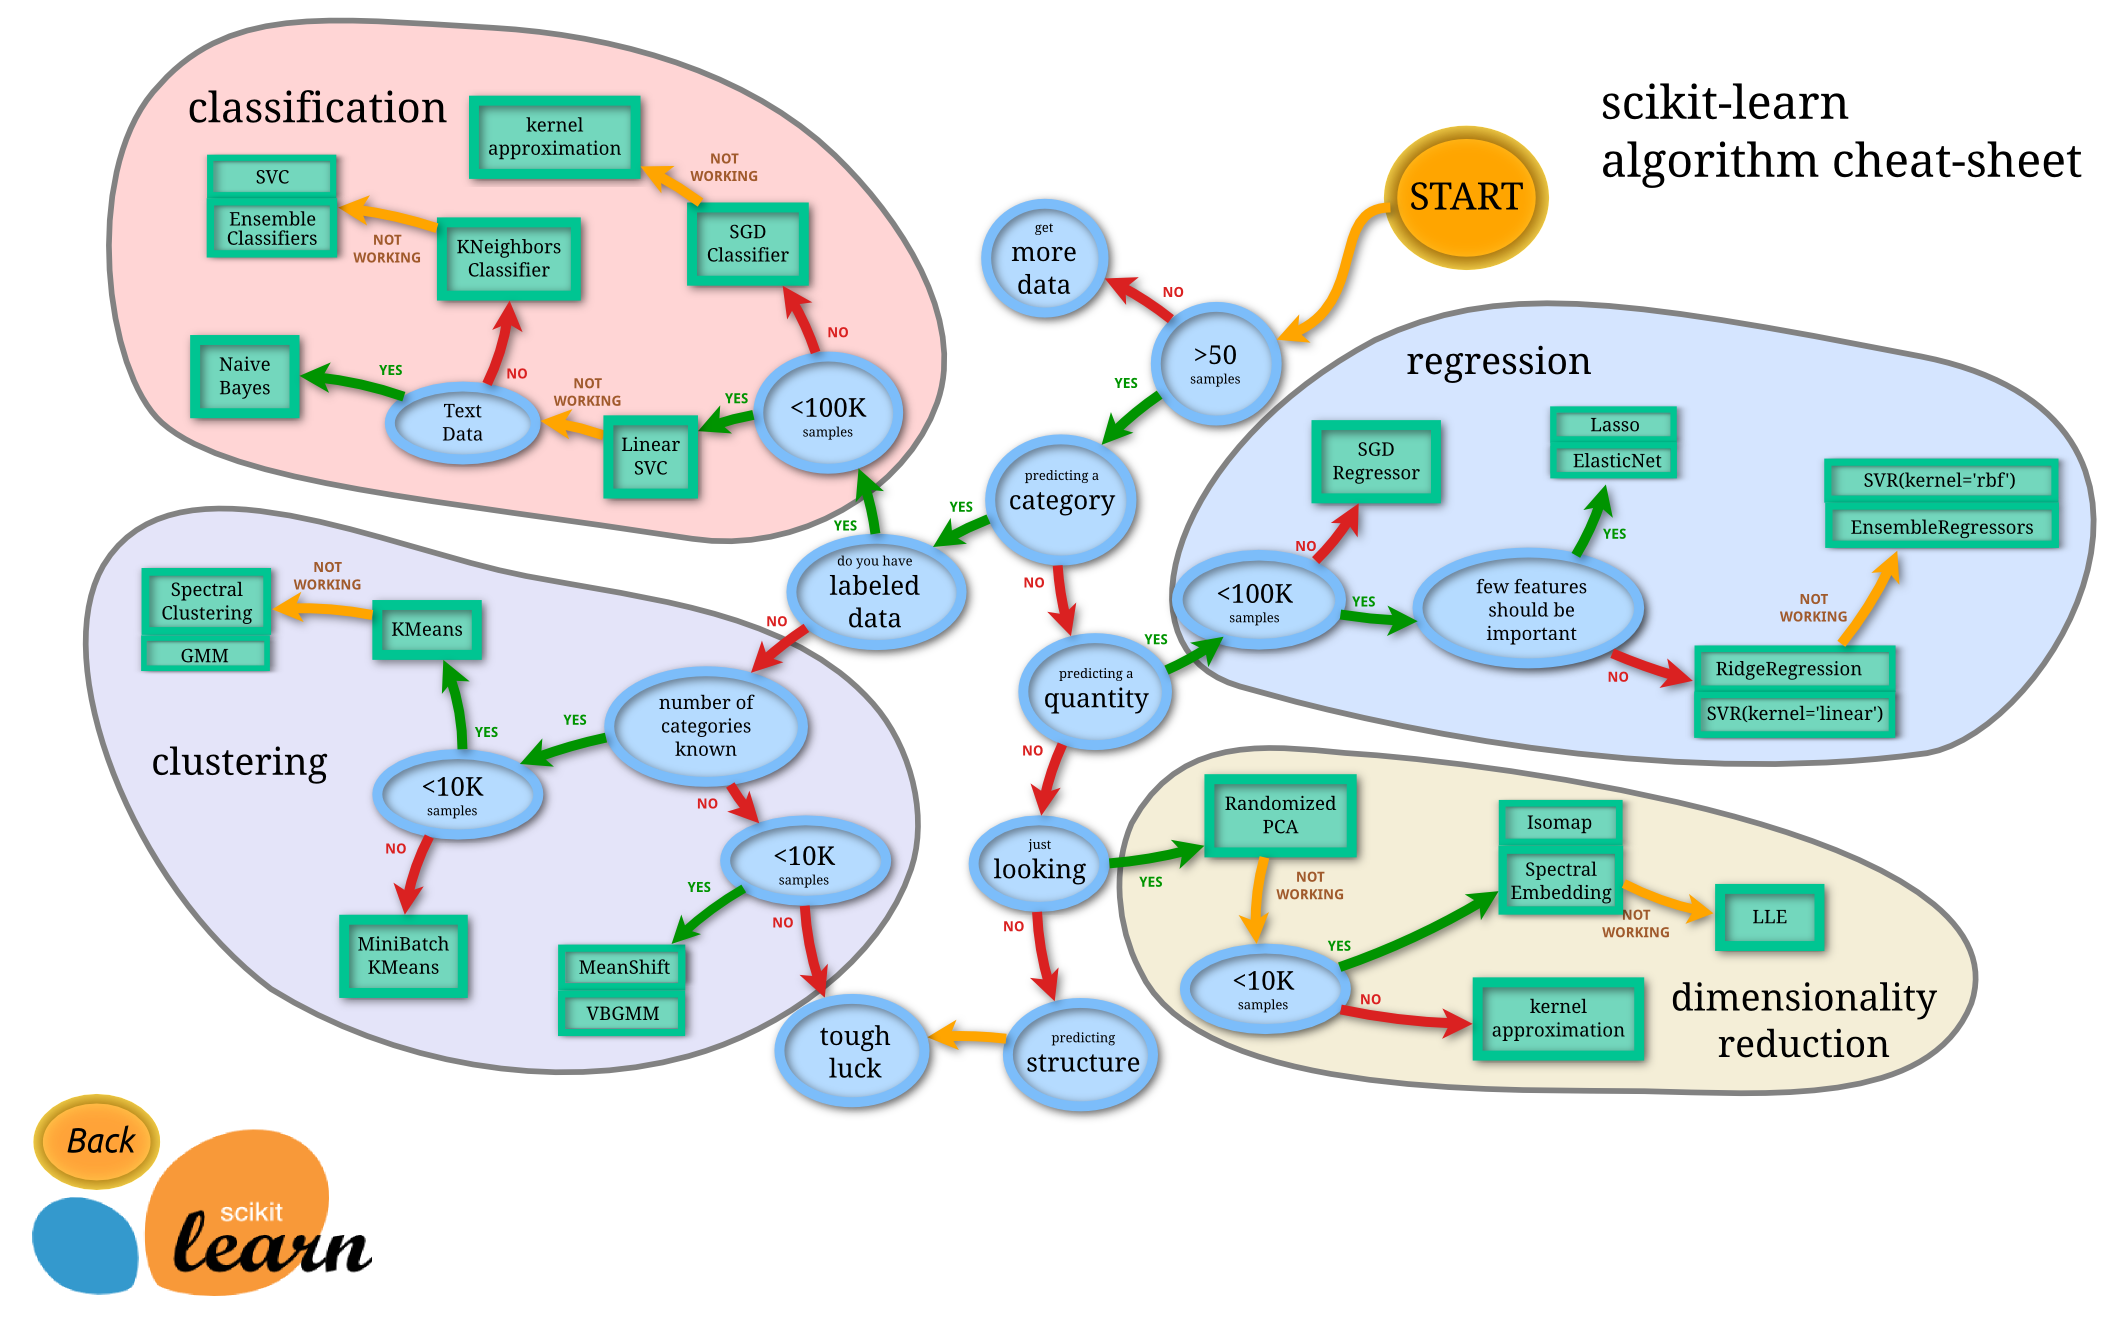
\includegraphics[width=\textwidth]{scheme_estimators.png}
	\caption{Esquema scikit-learn para la elección de un estimador}
	\label{fig:scheme_estimators}
\end{figure}


En nuestro caso contamos con más de 50 muestras, queremos predecir a que categoría pertenecen y contamos con los datos etiquetados gracias a la columna \textit{Attrition}.
Por tanto, nos encontramos en la burbuja \textit{classification} de la Figura \ref{fig:scheme_estimators}.
Y vamos a elaborar un proceso para decidir cual de ellos nos conviene más.\\

Para construir un modelo es necesario determinar las características que se van a usar, con que estimador se va a realizar la predicción y bajo que parámetros.

\subsection{Cálculo de la precisión de un modelo}
Una vez elegido el modelo existen distintas formas de evaluar dicho modelo. Esto es posible en problemas supervisados, como es nuestro caso en el que conocemos el resultado para ciertos datos.\\

Con el modelo elegido es necesario entrenarlo con un conjunto de datos. Si lo entrenamos con todos los datos con los que contamos, solo podremos realizar predicciones con muestras que pertenecen al conjunto de entrenamiento. Lo cual no es muy revelador, pues es normal que el modelo se comporte bien ante muestras con las cuales se le ha entrenado.\\

Para evitar caer en este error existe el método de separación de los datos en dos conjuntos, uno de entrenamiento y otro de pruebas. Este método es conocido como \textbf{Split Training}. Podemos ver esta separación en la Figura \ref{fig:splittraining}.\\

Este método consiste en separar los datos en dos conjuntos: uno de entrenamiento (\textit{train}), y otro de pruebas (\textit{test}).	
Se entrena al modelo con el conjunto de entrenamiento y se realiza la predicción con los datos de prueba. Una vez realizada la predicción se compara con el resultado correcto utilizando alguna sistema de puntuación (accuracy, f1, roc\_auc \ldots).


\begin{figure}[H]
\centering
\begin{tikzpicture}[every node/.append style={draw, rounded corners, inner sep=10pt}]
    \node [text width=3cm, text centered,rectangle split, rectangle split horizontal, rectangle split parts=2, rectangle split part fill={green!50, red!50}]
        {Training
		\nodepart{two} Test};
		 
\end{tikzpicture}
\caption{Split training}
\label{fig:splittraining}
\end{figure}

Sin embargo, puede que al hacer la separación en estos dos conjuntos se de un caso óptimo o por el contrario un caso fatal. Es por eso que se introduce otro nuevo método de evaluación, \textbf{Cross Validation} o Validación Cruzada.\\

Este método consiste en dividir los datos en una partición con $k$ conjuntos. Y realizar $k$ veces el método \textit{Split Training}. En cada iteración, el conjunto \textit{test} va siendo un elemento distinto de la partición y el conjunto \textit{train} lo forman los $k-1$ elementos restantes de la partición.
Una vez finalizadas cada una de las $k$ evaluaciones con \textit{Split training} se realiza la media de las puntuaciones obtenidas, dando lugar a la puntuación con \textit{Cross Validation}. Podemos ver un ejemplo en la Figura \ref{fig:crossvalidation}.


\begin{figure}
\centering
\begin{tikzpicture}
%[every node/.append style={draw, rounded corners, inner sep=10pt}]
\tikzset{
	block/.style={
		draw, rounded corners, inner sep=10pt,	
       text width=3cm, text centered,rectangle split, rectangle split horizontal, rectangle split parts=3
       }
}

    \node [block, rectangle split part fill={red!50, green!50, green!50}] (uno)
        {Test
         \nodepart{two} Training
		 \nodepart{three} Training};
		 
	\node [block, below=1cm of uno, rectangle split part fill={green!50, red!50, green!50}] (dos)
        {Training
         \nodepart{two} Test
		 \nodepart{three} Training};
		 
	\node [block, below=1cm of dos, rectangle split part fill={green!50, green!50, red!50}] (tres)
        {Training
         \nodepart{two} Training
		 \nodepart{three} Test};
		 
	\node[right=of uno] (num_uno){87\%};
	\node[right=of dos] (num_dos){92\%};
	\node[right=of tres](num_tres){88\%};
	\node[below=of num_tres] (num_total){89\%}
	(num_tres.south) -- coordinate (aux) (num_tres.south|-num_total.north);
	
	\draw ([xshift=-1cm]num_total.north west|-aux) -- ([xshift=1cm]num_total.north east|-aux);   
		 
\end{tikzpicture}
\caption{Evaluación con el método \textit{Cross Validation} con $k=3$}
\label{fig:crossvalidation}
\end{figure}


\subsection{Selección de características}
Esta fase consiste en la elección de aquellas características que aporten más información, para poder ser usadas en los distintos estimadores.
Una pregunta común sería, ¿Por qué no usamos todas las características para realizar la predicción? La respuesta es sencilla, y es que en este caso, más no significa mejor.
Usar características que no aportan información e introducen ruido en los datos repercute negativamente en la precisión del modelo.\\


La librería \textit{scikit-learn} proporciona mecanismos para la selección automática de características.
Estos son los que hemos usado:

\begin{itemize}
\item \textbf{Recursive Feature Elimination}. Dado un estimador que asigne pesos a las características RFE comienza con todas las características y recursivamente va considerando conjuntos más pequeños de características.
Si usamos la clase \texttt{sklearn.feature\_selection.RFECV} de \textit{scikit-learn} podemos realizar este proceso de eliminación encontrando el número óptimo de características.

\item \textbf{Feature selection}. Únicamente puede ser usado con estimadores que asigna importancia a las características tras ser entrenado. Podemos hacer uso de este método de selección de características gracias a la clase \texttt{sklearn.feature\_selection.SelectFromModel} de \textit{scikit-learn}.

\end{itemize}

\subsection{Optimización de parámetros}
Una vez elegido un estimador, es necesario configurar los parámetros para obtener el mejor resultado posible con dicho estimador. Para ello existe una clase en \textit{scikit-learn} llamada \texttt{sklearn.model\_selection.GridSearchCV} a la cual le podemos pasar como argumentos un diccionario de \textit{python} con los valores que debe explorar para cada uno de los parámetros del estimador. Y lo que hace \textit{gridSearchCV} es ejecutar \textit{Cross Validation} para las distintas combinaciones de parámetros.
Una vez finalizadas, podemos acceder tanto a la puntuación más alta como a los parámetros del estimador que han dado lugar a dicha puntuación.


\subsection{Selección del estimador}
Los diferente estimadores que he probado son:

\begin{itemize}
\item \textbf{Linear Support Vector Classification}. Perteneciente a la familia de estimadores \textit{lineales}, cuyo objetivo es la construcción de un hiperplano en el espacio donde se encuentran los datos. De manera que un punto se clasificará dependiendo de a que lado del hiperplano se encuentre.

\item \textbf{K-vecinos más cercanos o K nearest neighbors Classifier}. Este estimador tiene como parámetros un valor $k$ que indica el número de vecinos en los que debe fijarse y otro parámetro \textit{weight\_options} que puede tomar los valores \textit{uniform} y \textit{distance}.
A la hora de clasificar un punto el estimador se fija en los $k$ puntos de entrenamiento más cercanos, detecta que clase es la más común en esos $k$ puntos, y esa clase es el resultado de la predicción. Cuando el parámetro \textit{weight\_options} tiene el valor \textit{distance} se ponderan los valores de los $k$ vecinos con el inverso de la distancia al punto que deseamos clasificar.

\item \textbf{Regresión logística} se trata de un tipo de análisis de regresión usado para predecir el resultado de una variable categórica.

\end{itemize}


El resultado de todo el proceso ha dado lugar al modelo formado por el estimador Regresión logística, con las características obtenidas tras aplicar el método de \textit{Recursive Feature Elimination}. Resultando ser 42 el número óptimo de características.\\

La búsqueda de los parámetros con \textit{GridSearchCV} ha dado lugar a la siguiente configuración.\\

%['OverTime_Yes', 'YearsAtCompany', 'JobInvolvement', 'JobLevel', 'JobSatisfaction', 'NumCompaniesWorked', 'BusinessTravel_Travel_Rarely', 'BusinessTravel_Travel_Frequently', 'Department_Research & Development', 'Department_Sales', 'EducationField_Life Sciences', 'EducationField_Marketing', 'EducationField_Medical', 'EducationField_Other', 'EducationField_Technical Degree', 'EnvironmentSatisfaction', 'Gender_Male', 'JobRole_Human Resources', 'JobRole_Laboratory Technician', 'JobRole_Manager', 'JobRole_Manufacturing Director', 'JobRole_Research Director', 'JobRole_Research Scientist', 'JobRole_Sales Executive', 'JobRole_Sales Representative', 'MaritalStatus_Single', 'MaritalStatus_Married', 'PerformanceRating', 'RelationshipSatisfaction', 'StockOptionLevel', 'TrainingTimesLastYear', 'WorkLifeBalance', 'YearsInCurrentRole', 'YearsSinceLastPromotion', 'YearsWithCurrManager', 'Age_Over', 'Income_Over', 'Distance_Over', 'AtCompany_Over', 'OverTime_Balance', 'YearsPerCompany', 'YearsAtCurrRole_Rate']

\begin{lstlisting}[language=python, breaklines]
	LogisticRegression(penalty= 'l2',C=1, fit_intercept=True, intercept_scaling=0.1, tol=0.001, class_weight=None)
\end{lstlisting}

Proporcionando una precisión de 89,38 \%\\


Ahora que hemos elegido el modelo que vamos a usar para realizar las predicciones, tenemos que entrenarlo con todos los datos con los que contamos (con los 1470 empleados).
De modo que podremos realizar predicciones sobre datos que esten fuera de nuestra población inicial, teniendo el modelo entrenado lo máximo posible.\\











	\chapter{Conclusiones}

El desarrollo de la \iface{} se ha realizado satisfactoriamente. Sirviendo como un proyecto de integración interno para \acrshort{bnb}.

La salida a producción de \wday{} se realizó el 4 de abril de 2017. Con ello los sistemas de integración, incluyendo la \iface{} se pusieron en funcionamiento.\\


%Integración

Con este trabajo de fin de grado he podido comprobar la versatilidad del lenguaje \textit{python} a la hora de construir micro-servicios que se comunican con varias aplicaciones.
También he podido entender que no es posible tener todo unificado en una misma aplicación. Por ello es necesario la integración de múltiples aplicaciones, para conseguir que los datos estén sincronizados.
He visto la variedad de metodologías utilizadas por distintas aplicaciones para facilitar las integraciones: servicios web, APIs\ldots
También he comprobado las diferentes formas de permitir el acceso a las funcionalidades de integración: OAuth2.0 y acceso por usuario y contraseña.\\


%Analisis de datos

En la parte del estudio de los datos de los trabajadores de una empresa, he podido comprobar las ventajas que presenta el lenguaje \textit{python} tanto para el análisis de datos como para realizar \textit{Machine Learning}.
A pesar de no haber usado lenguajes como \textit{R} o \textit{Scala} puedo asegurar que python es una buena opción cuando se trata con proyectos de \textit{Machine Learning}.\\


Ahora vamos a ir comprobando uno a uno los objetivos establecidos en el capítulo de introducción, para ver si se han cumplido.

\begin{itemize}
	\item Desarrollar un microservicio que realice la integración entre \hs{} y \wday{}.\\
	
		Este objetivo se ha conseguido.
	\item Conseguir que al introducir datos en \hs{}, automáticamente se sincronicen con \wday{}.\\
	
	Una vez que se crea un \textit{deal} en \hs{},si corresponde se crea automáticamente un proyecto en \wday{}.
	
	\item Que al modificar datos en \hs{}, se modifiquen en \wday{} de forma automática.\\
	
	Cuando un \textit{deal} es modificado en \hs{}, que tiene un \textit{project} asociado en \wday{}, el \textit{project} asociado también se ve modificado. Esta sincronización ocurre con la modificación de cualquiera de las propiedades de un \textit{deal}, incluso si modificamos el objeto \textit{company} asociado.
	
	\item Que la integración sea rápida, y el tiempo transcurrido entre la introducción o cambio de datos en \hs{} y los cambios en \wday{} sea el mínimo posible.\\
	Se ha conseguido que la integración sea instantánea gracias a las suscripciones a los \textit{webhook} de \hs{}. 
	Se ha evitado así la creación de un proceso recurrente que compruebe periódicamente si ha habido algún cambio en \hs{}. 
	
	\item La integración ha de ser segura. Estar provista de mecanismos para evitar posible ataques de terceras personas.\\
	
	Se ha conseguido garantizar la seguridad del sistema, añadiendo comprobaciones sobre los mensajes recibidos para asegurar su procedencia.
	
	\item La integración debe ser totalmente transparente para el usuario.\\
	
	El usuario no necesita saber como funciona la integración. Simplemente creando o modificando objetos en \hs{} consigue que la información se sincronice en \wday{}.
	Sin embargo los usuarios deben tener presente en que fases un \textit{deal} es sincronizado y en que fases se excluye de la sincronización.
	
	\item El programa no debe abortar su ejecución de manera inesperada.\\
	
	Gracias al \textit{framework} utilizado \textit{web.py}, no es posible que el programa finalice su ejecución de forma inesperada. 
	Ya que internamente \textit{web.py} captura todas las excepciones y las muestra por consola. En cualquier caso, se ha intentado en la medida de lo posible controlar todos los tipos de errores y excepciones que pudiesen ocurrir.
	
	\item En la medida de lo posible evitar errores en la introducción de datos. Evitar que se cree información duplicada.\\
	
	Este objetivo no se ha podido llevar a cabo, ya que la duplicación de la información en \hs{} es un error del usuario. Si el usuario no se da cuanta de la existencia de un \textit{deal} o \textit{company} puede crear uno duplicado y que consecuentemente se sincronice, cuando eso no es el resultado esperado.
	
	
	\item El servicio que realiza la integración tiene que estar en ejecución ininterrumpida.\\
	
	La \iface{} se encuentra en ejecución en un servidor externo, activo todo el tiempo.
	
	\item Evitar la pérdida de datos.\\
	
	Para evitar la pérdida de datos se ha creado un proceso que revisa todos los \textit{deals} e integraría aquellos \textit{deals} que no están integrados. 
	Ya sea debido a una interrupción del servicio o la pérdida de algún mensaje.
	
	Sin embargo no se ha podido comprobar el correcto funcionamiento de este proceso.
	\item Localmente se debe llevar la cuenta de los datos que se encuentran integrados.\\
	
	Se ha conseguido mediante el uso de una base de datos sencilla.
	Sin embargo no está totalmente protegida de errores  de los usuarios, pues por ejemplo si un \textit{deal} se pase a la fase de cierre por equivocación, se para la sincronización del mismo.
	De manera que es necesario un cambio manual en la tabla de \textit{deals} excluidos.
	
	\item El servicio debe soportar ser reiniciado.\\
	
	Gracias al almacenamiento persistente de los \textit{token}, es posible reiniciar el sistema sin problemas de funcionamiento. No obstante es posible que problemas de pérdidas de datos tengan lugar y sea necesario tomar medidas(Como por ejemplo ejecutar el proceso que revisa todos los \textit{deals}).
	\item El prototipo predictor debe ser capaz de decidir si es muy probable que un empleado abandone la empresa.\\
	
	Este objetivo se ha cumplido, aunque quizá se podría haber alcanzado mejores resultados haciendo uso de datos más fiables.
	\item Concluir que datos son más importantes para predecir el abandono en el trabajo.\\
	
	Hemos podido averiguar que datos son determinantes a la hora de predecir las rotaciones en la plantilla de una empresa.
	\item Poder tomar mediadas de acuerdo a las conclusiones a las que se llegue para elaborar mejores predicciones.\\
	
	Gracias a la información obtenida con el estudio y la predicción, se ha podido recomendar medidas de actuación que reduzcan estos sucesos en las empresas.
\end{itemize}






	
	
	\input{Others/bibliography	.tex}
	
	%\printglossary[type=\acronymtype]
	\printglossary[type=\acronymtype, title=Acrónimos,toctitle=Acrónimos]
 
	\printglossary

\end{document}


